%%%%%%%%%%%%%%%%%%%%%%%%%%%%%%%%%%%%%%%%%%%%%%%%%%%%%%%%%%%%%%%%%%%%%%%%%%%%%%%
% $Id$
%
% Documentation file for the BYU-LANL Triple Modular Redundancy (BL-TMR) Tool.
%
% Author: Brian Pratt <bhpratt@gmail.com>
%         James Carroll <jcarroll@byu.net>
%         Jonathan Johnson <jonjohn@byu.net>
%%%%%%%%%%%%%%%%%%%%%%%%%%%%%%%%%%%%%%%%%%%%%%%%%%%%%%%%%%%%%%%%%%%%%%%%%%%%%%%

\documentclass[english]{article}
%\usepackage[T1]{fontenc}
\usepackage{fullpage}
\usepackage{amsmath}
\usepackage{epsfig}
\usepackage{graphicx}
\usepackage{verbatim}
\usepackage{moreverb}
\numberwithin{figure}{section}
%\usepackage[latin1]{inputenc}
\IfFileExists{url.sty}{\usepackage{url}}
                      {\newcommand{\url}{\texttt}}
% use this instead of pdfgraphcompat
% Check for PDFLaTeX
\newif\ifpdf 
\ifx\pdfoutput\undefined 
   \pdffalse % we are not running PDFLaTeX 
\else
   \pdfoutput=1 % we are running PDFLaTeX 
   \pdftrue 
\fi


% This processes the file using the 'hyperref.sty' package when
% PDFLaTeX is used.  This adds internal hyperlinks throughout the
% document in the generated PDF.
\ifpdf
   \usepackage[colorlinks={true},
     urlcolor=rltblue,       % \href{...}{...} external (URL)
     filecolor=rltgreen,     % \href{...} local file
     linkcolor=rltred,       % \ref{...} and \pageref{...}
     pdftitle={BYU-LANL Triple Modular Redundancy Usage Guide Version 0.5.0 -
     20 May, 2009}, % pdfauthor={BYU Configurable Computing Lab},%
     pdfproducer={pdfLaTeX},%
     %pdfadjustspacing=1,
     pdftex]{hyperref}
\fi

% Define colors used by hyperref
\usepackage{color}
\definecolor{rltred}{rgb}{0.75,0,0}
\definecolor{rltgreen}{rgb}{0,0.5,0}
\definecolor{rltblue}{rgb}{0,0,0.75}


\vfuzz2pt % Don't report over-full v-boxes if over-edge is small
\hfuzz2pt % Don't report over-full h-boxes if over-edge is small

% 1: label, 2: path, 3: filename except extension (minus .png or .eps), 4: caption
\newcommand\figurecaption[4]{
\begin{figure}[ht]
  \centering
  \includegraphics[width=1.0\linewidth]{#2/#3}
  \parbox{1.0\linewidth}{\caption{\label{#1}#4}}
\end{figure}
}

\makeatletter

%%%%%%%%%%%%%%%%%%%%%%%%%%%%%% LyX specific LaTeX commands.
%% Bold symbol macro for standard LaTeX users
\providecommand{\boldsymbol}[1]{\mbox{\boldmath $#1$}}

\usepackage{babel}
\makeatother

\title{BYU-LANL Triple Modular Redundancy \\ Usage Guide \\  }
  
\author{Brigham Young University \\ Configurable Computing Lab}

\date{\today}

\begin{document}

\maketitle

\newpage
\tableofcontents
\newpage

\section{Toolflow Illustration}
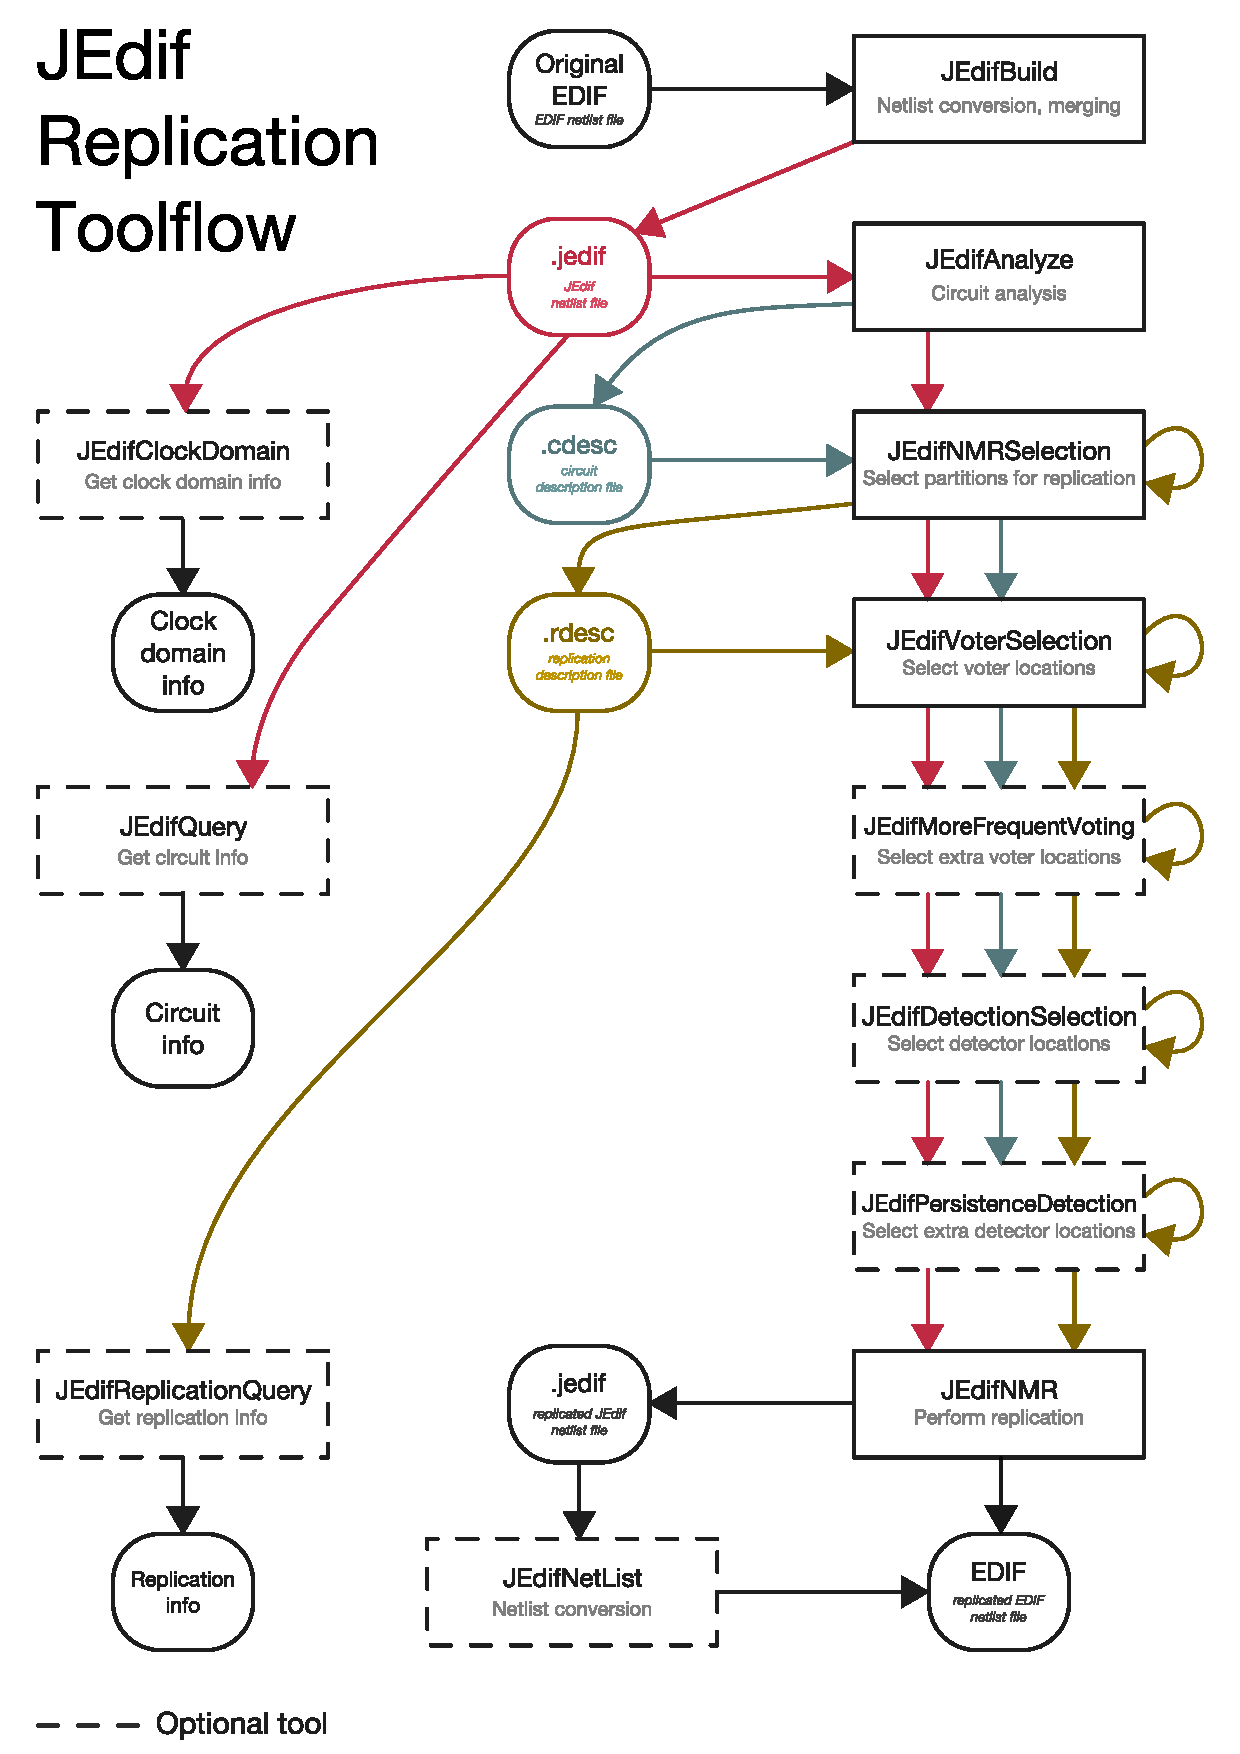
\includegraphics[scale=0.7]{tool_flow.pdf}
\newpage


%%%%%%%%%%%%%%%%%%%%%%%%%%%%%%%%%%%%%%%%%%%%%%%%%%%%%%%%%%%%
\section{Introduction}
The BYU-LANL Triple Modular Redundancy (BL-TMR) Tool is an EDIF-based
tool to insert redundancy in an FPGA design in order to increase
reliability. Triple modular redundancy (TMR) and/or duplication with
compare (DWC) are applied to an EDIF input file according to the
options chosen by the user. Partial replication focuses on ``persistent''
components of the design in order to get the ``most bang for your buck.''

The tool is also capable of inserting detectors for doing error detection using
DWC. Single- and dual-rail error detectors can be inserted in both triplicated
and duplicated designs. Special persistence detectors can be inserted in order
to give the ability to classify detected errors as persistent or non-persistent.

\section{Replication Toolflow}
The tool is split into several subtools. This allows the user to
adjust various command-line options in one phase, and then move onto
the next phase. Some phases such as JEdifNMRSelection are designed to be run in
passes in order to obtain the desired results. For example, in order to mix
duplication and triplication in a design, you can run JEdifNMRSelection twice,
once to select partitions to triplicate, and once more to select partitions to
duplicate.

\subsection{JEdifBuild}
JEdifBuild creates merged netlists in a .jedif file format from
multiple .edf files. By default, JEdifBuild also flattens the design
and optionally performs FMAP removal, RLOC removal, SRL replacement,
and half-latch removal (functions performed by JEdifSterilize in
previous versions of the toolflow). The .jedif file format is an
intermediate file format used by the remainder of the replication
tools.

\subsection{JEdifAnalyze}
JEdifAnalyze performs some basic circuit analysis necessary for
subsequent executables. In particular, it performs feedback and IOB
analysis. The results of JEdifAnalyze are saved in a circuit
description file (.cdesc) required by later executables.

\subsection{JEdifNMRSelection}
JEdifNMRSelection determines which parts of a design will be
replicated. This executable can be run in multiple passes to select
different parts of a design for different kinds of replication. Each
run of JEdifNMRSelection can select portions of a design for a single
replication type (i.e. duplication, triplication). Design portions can
be selected for replication based on available space or specific cell
types, instances, ports, and clock domains specified by the user. The
results of JEdifNMRSelection are saved in a replication description
(.rdesc) file. This file can be modified by subsequent runs of this
and other executables in the toolflow.

\subsection{JEdifVoterSelection}
JEdifVoterSelection determines the locations where voters will be
inserted into a triplicated design (or triplicated portions of a
design). Voter locations are determined using a feedback cutset
algorithm and rules for voting where downscaling is necessary. The
results are added into the replication description (.rdesc) file.

\subsection{JEdifMoreFrequentVoting}
\emph{Optional:} JEdifMoreFrequentVoting inserts extra voters for more frequent voting within a design based on a logic levels threshold or a total number of desired
partitions.

\subsection{JEdifDetectionSelection}
\emph{Optional:}
JEdifDetectionSelection determines detector locations for both triplicated and
duplicated design portions using user-specified options. Like
JEdifNMRSelection, this tool is designed to be run in multiple passes
(only one replication type can be processed per pass). Results are
saved in the replication description file (.rdesc).

\subsection{JEdifPersistenceDetection}
\emph{Optional:} JEdifPersistenceDetection determines additional
detector locations necessary for classifying persistent/non-persistent
errors detected in a design. It is designed to be run in multiple
passes. Results are saved in the replication description (.rdesc) file.

\subsection{JEdifNMR}
JEdifNMR performs the replication selected by previously run
tools. Information about what to replicate and where to insert
voters/detectors is obtained from the replication description (.rdesc)
file created by the previous steps.

\subsection{Other JEdif tools}

\subsubsection{JEdifNetList}
JEdifNetlist converts a netlist in .jedif format to EDIF (.edf) format for use
with other standard EDIF tools.

\subsubsection{JEdifQuery}
JEdifQuery is a tool used to query the contents of a .jedif file and
to provide summary information about the EDIF design contained within.

\subsubsection{JEdifReplicationQuery}
JEdifReplicationQuery is a tool used to query the contents of a
replication description file (.rdesc) and provide summary information
about the kind of replication that will be performed on a design. It
reports information about replication types, organs to be inserted
(i.e. voters, detectors), and detection error outputs.

\subsubsection{JEdifClockDomain} 
The JEdifClockDomain tool is a .jedif based tool to analyze FPGA
designs to obtain information about the clock(s). The tool first
identifies all clocks in a design. This information is then used to
optionally display other information, such as classifying Xilinx
primitives into one or more domains, showing clock crossings, etc.

%%%%%%%%%%%%%%%%%%%%%%%%%%%%%%%%%%%%%%%%%%%%%%%%%%%%%%%%%%%%
\newpage
\section{JEdifBuild Options}
JEdifBuild creates merged netlists in a .jedif file format from
multiple .edf files. By default, JEdifBuild also flattens the design
and optionally performs FMAP removal, RLOC removal, SRL replacement,
and half-latch removal (functions performed by JEdifSterilize in
previous versions of the toolflow). The .jedif file format is an
intermediate file format used by the remainder of the replication
tools.

Although flattening occurs by default, it can be disabled with the
\texttt{--no\_flatten} option. It is also possible to specify that specific
cell types should not be flattened. This can be accomplished by adding a
\texttt{`do\_not\_flatten'} property to the cell in the .edf file as follows:\\
\texttt{(property do\_not\_flatten (boolean (true)))}

If this property is used on a cell that is a black box in the main design file
and is merged in from a separate .edf or .edn file, the property should be
specified in the black box \emph{definition} file, not in the main design .edf
file.

It should be noted that designs that are not flattened will not be replicated
properly. Any unflattened cells will be replicated as an atomic unit,
preventing proper voter insertion. Use the \texttt{`do\_not\_flatten'} property
only when this is the desired behavior.

Cell types that are selected as pre-mitigated cells using \texttt{`port\_group'}
properties (see Section~\ref{sec:pre-mitigation}) are also left unflattened.
Flattening for pre-mitigated cells is not necessary since they will not be replicated.

Options can be specified on the command line or in a configuration file in any 
order. This section describes each of these options in detail.

\begin{verbatim}
> java edu.byu.ece.edif.jedif.JEdifBuild --help
Options:
  [-h|--help]
  [-v|--version]

  <input_file>
  [(-o|--output) <output_file>]
  
  [(-d|--dir) dir1,dir2,...,dirN ]
  [(-f|--file) file1,file2,...,fileN ]

  [--no_flatten]
  [--no_open_pins]
  [--blackboxes]
  [--no_delete_cells]
  [--pack_registers <{i|o|b|n}>]

  [--replace_luts]
  [--remove_fmaps]
  [--remove_rlocs]
  [--remove_hl]
  [--hl_constant <{0|1}>]
  [--hl_use_port <hl_port_name>]
  [--hl_no_tag_constant]

  [(-p|--part) <part>]

  [--write_config <config_file>]
  [--use_config <config_file>]

  [--log <logfile>]
  [--debug[:<debug_log>]]
  [(-V|--verbose) <{1|2|3|4|5}>]
  [--append_log]
\end{verbatim}

%%%%%%%%%%%%%%%%%%%%%%%%%%%%%%%%%%%%%%%%%%%%%%
\subsection{File options: input, output, etc.}
The following options specify the top-level input EDIF file, any auxiliary EDIF
files, and the destination EDIF file.

\subsubsection{\texttt{<input\_file>}}
Filename and path to the EDIF source file containing the top-level cell to be 
converted. This is the only required parameter.

Allowed filename extensions are:
\begin{itemize}
  \item Parsable Edif: edn,edf,ndf
  \item Binary Edif (Blackboxes): ngc,ngo
  \item Blackbox Utilization: bb
\end{itemize}

Parsable EDIF files will be parsed and included in the algorithms.
Binary EDIF files are not parsable, but the program recognizes them as
blackboxes, and will not complain about not finding the entity.
Blackbox utilization files allow the user to specify the resource use
of the blackboxes to help in the utilization estimate and partial tmr
algorithms.  The file format is ``Resource:Number''.  Below is an
example:

myblackbox.bb:\\
\begin{verbatim}
  BRAM:1
  FF:400
  LUT:100
\end{verbatim}

This entity, named myblackbox uses 1 BRAM, 400 Flipflops and 100 LUTS

\subsubsection{\texttt{(-o|--output) <output\_file>}}
Filename and path to the jedif output file.

Default: \texttt{<input file>.jedif} in the current working directory.

\subsubsection{\texttt{(-d|--dir) dir1,dir2,\ldots,dir3}}
Comma-separated list of directories containing external EDIF files referenced 
by the top-level EDIF file. The current working directory is included by 
default and need not be specified. There can be multiple \texttt{-d} options.

Example: \texttt{-d aux\_files,/usr/share/edif/common -d
  moreEdifFiles/}

\subsubsection{\texttt{(-f|--file) file1,file2,\ldots,fileN}}
Similar to the previous option, but rather than specifying directories to 
search, each external EDIF file is named explicitly---including the path to the 
file. There can be multiple \texttt{-f} options. 

Example: \texttt{-f multBox.edn,src/adder.edf -f /usr/share/edif/blackBox.edf}.

\subsection{Maintenance Options}
The following options allow some control over that happens during the 
conversion process
  
\subsubsection{\texttt{--no\_flatten}}
By default JEdifBuild will flatten the EDIF files. Flattening is required by the 
TMR tools, but other applications my wish to keep the hierarchical
design. 

\subsubsection{\texttt{--no\_open\_pins}}
Do not allow the parser to infer open pins on black box definitions.

\subsubsection{\texttt{--blackboxes}}
Allow parser to continue if blackbox definitions are not found.

\subsubsection{\texttt{--no\_delete\_cells}}
By default JEdifBuild will remove unused cells, to reduce the size of the final
.jedif file. However, the user can request that these cells be retained for 
future use.

\subsubsection{\texttt{--pack\_registers} \{i\textbar o\textbar b\textbar n\}}
By default, the BL-TMR tool treats all ports on the input EdifCell as top-level
ports (those that will be the inputs and outputs of the FPGA). The half-latch 
tool must therefore treat any FFs that will be packed into the IOBs differently
than other FFs (at least with Virtex devices). This option allows the user to
specify which IOBs the registers should be packed into: inputs (\emph{i}),
outputs (\emph{o}), both (\emph{b}), or none (\emph{n}). The default is to pack
both input and output registers.

\subsection{Sterilize Options}

\subsubsection{\texttt{--replace\_luts}}
By default JEdifBuild will not remove LUT RAMs acting as SRLs in the design.  These
LUT RAMs can cause problems as they are not scrubbable.  This option tells the 
tool to replace these LUT RAMs with actual SRLs.

\subsubsection{\texttt{--remove\_fmaps}}
Remove FMAPS from the input design.

\subsubsection{\texttt{--remove\_rlocs}}
Setting this option will tell JEdifBuild to remove ALL RLOCs in the design.
The replication tools will not work correctly if a design contains RLOCs.

\subsubsection{\texttt{--remove\_hl}}
Remove half-latches in the input design before performing TMR.

Note: Not \emph{all} half-latches can be removed at the EDIF 
level for all architectures. Some post-processing may be necessary.

\subsubsection{\texttt{--hl\_const} $\{0,1\}$}
Sets the polarity of the half-latch constant to be used, whether an 
internally-generated constant or a top-level port. 

Valid options are \texttt{0} and \texttt{1}. Default: \texttt{0}.

\subsubsection{\texttt{--hl\_use\_port <hl\_port\_name>}}
Specify a top-level port to use in place of half-latches when 
using half-latch removal. The top-level port will have the name specified with 
this option and the polarity (1 or 0) specified with the \texttt{--hlConst} 
option.

\subsubsection{\texttt{--hl\_no\_tag\_constant}}
When half-latch removal is used, a constant comes from either a constant
generator cell (ROM$16$X$1$) or a port specified by the user. In either case,
the input buffer for the port or the generator cell should be triplicated (or
duplicated) to ensure reliability. By default, such instances are tagged with
an EDIF property called 'half\_latch\_constant' so that they can be
automatically selected for replication by JEdifNMRSelection later in case
partial replication is used. This option disables the default behavior of
tagging safe constant instances.

\subsection{Target Technology and Part Options}

\subsubsection{\texttt{--technology <techname>}}
Target architecture for the triplicated design. Used to take into account 
various technology-specific properties. This argument is \emph{not} 
case-sensitive.

Valid technologies: \texttt{Virtex} and \texttt{Virtex2}. Default: 
\texttt{Virtex}.

\subsubsection{\texttt{--part <partname>}}
Target architecture for the triplicated design. Used to take into account 
part-specific properties, including the number of resources available 
in each part. Valid parts include all parts from the \emph{Virtex} and 
\emph{Virtex2} product lines, represented as a concatenation of the part name 
and package type. For example, the ``Xilinx Virtex 1000 FG680'' is represented 
as \texttt{XCV1000FG680}. This argument is \emph{not} case-sensitive.

Default: \texttt{xcv1000fg680}.
% TODO: Add list of all supported part numbers. All parts listed in
% XilinxVirtexDeviceUtilizationTracker.java and
% XilinxIIVirtexDeviceUtilizationTracker.java

%%%%%%%%%%%%%%%%%%%%%%%%%%%%%%%%%%%%%%%%%%%%%%
\subsection{Configuration File Options}
\label{config options}
The BLTmr tools can use configuration files in place of command-line parameters. 
If a parameter is specified in a configuration file, it will be passed to the 
BLTmr tool, unless it is overridden by the same argument on the command-line. 

\subsubsection{\texttt{--useConfig <config\_file>}}
\label{useConfig}
Specify a configuration file from which to read parameters.

\subsubsection{\texttt{--writeConfig[:<config\_file>]}}
Write the current set of command-line parameters to a configuration file and 
exit. The parameters will be parsed to ensure they are valid, but the BLTmr tool
will not run.  Note that only the parameters on the command-line are stored in
the configuration file. When using \texttt{--writeConfig}, any use of
\texttt{--useConfig} is ignored. This is to prevent complicated cascades
of configuration files combined with command-line options.

Examples:
\begin{itemize}
  \item \texttt{--writeConfig:JonSmith.conf} will write the command-line 
  parameters to the file \texttt{JonSmith.conf} in the current directory.
  \item \texttt{--writeConfig:/usr/lib/BLTmr/common.conf} will write the
  command-line parameters to the file \texttt{/usr/share/BLTmr/common.conf}. 
  \item See section \ref{using config}, ``Using Configuration Files,'' for
  more information.
\end{itemize}

\subsection{Logging options}

\subsubsection{\texttt{--log <logfile>}}
Specifies a file for logging output (default: sterilize.log)

\subsubsection{\texttt{--debug[:<debug\_log>]}}
Specifies a file for logging the debuggin output.If no file
specified, debug output is printed to the log file.

\subsubsection{\texttt{(-V|--verbose) <$\{1|2|3|4|5$\}>}}
Sets the verbosity level:
1 prints only errors, 
2 warnings, 
3 normal, 
4 log to stdout. 
5 prints debug information. 
(default: 3)

\subsubsection{\texttt{--append\_log }}
Append to the logfile instead of replacing it.


%
% Words to be ignored by the spell-checker:
%

% LocalWords:  BYU LANL BL-TMR EDIF FPGA TMR OBUF IBUF BUFG IBUFG LUTs
% LocalWords:  SCC SCCs FFs UCF Xilinx java JHDL netlister IOB IBUFs
% LocalWords:  OBUFs logfile INOUT TMR'd tmr txt JEdifBuild jedif edn edf dir



\newpage
\section{JEdifAnalyze}
JEdifAnalyze performs some basic circuit analysis necessary for
subsequent executables. In particular, it performs feedback and IOB
analysis. The results of JEdifAnalyze are saved in a circuit
description file (.cdesc) required by later executables.

The following options control the feedback and IOB analysis
performed by this executable. The results of the analysis
affect the execution of later steps in the toolflow.

\begin{verbatim}
>java edu.byu.ece.edif.jedif.JEdifAnalyze
Options:
  [-h|--help]
  [-v|--version]

  <input_file>
  (-o|--output) <output>

  [--pack_registers <{i|o|b|n}>]
  [--use_bad_cut_conn]
  [--no_iob_feedback]

  [(-p|--part) <part>]

  [--write_config <config_file>]
  [--use_config <config_file>]

  [--log <logfile>]
  [--debug[:<debug_log>]]
  [(-V|--verbose) <{1|2|3|4|5}>]
  [--append_log]
\end{verbatim}

%%%%%%%%%%%%%%%%%%%%%%%%%%%%%%%%%%%%%%%%%
\subsection{File Options}

\subsubsection{\texttt{<input\_file>}}
Filename and path to the jedif source file to be analyzed

\subsubsection{\texttt{(-o|--output) <output\_file>}}
Filename and path to the ciruit description file (.cdesc) that will be output.

\subsection{Analysis Options}
\subsubsection{\texttt{--pack\_registers} \{i\textbar o\textbar b\textbar n\}}
By default, the BL-TMR tool treats all ports on the input EdifCell as top-level
ports (those that will be the inputs and outputs of the FPGA). The half-latch 
tool must therefore treat any FFs that will be packed into the IOBs differently
than other FFs (at least with Virtex devices). This option allows the user to
specify which IOBs the registers should be packed into: inputs (\emph{i}),
outputs (\emph{o}), both (\emph{b}), or none (\emph{n}). The default is to pack
both input and output registers.

\subsubsection{\texttt{--use\_bad\_cut\_conn}}
Use bad cutgroup connectivity graph

\subsubsection{\texttt{--no\_iob\_feedback}}
Use this option to exclude IOBs from the feedback analysis. This is useful when
a top-level inout port is involved in feedback but by design will never be 
written to and read at the same time. Thus there is no \emph{real} feedback.
Using this option may greatly reduce the amount of feedback found in the design
and thus reduce the number of voters inserted.

\subsection{Target Technology and Part Options}

\subsubsection{\texttt{--technology <techname>}}
Target architecture for the triplicated design. Used to take into account 
various technology-specific properties. This argument is \emph{not} 
case-sensitive.

Valid technologies: \texttt{Virtex} and \texttt{Virtex2}. Default: 
\texttt{Virtex}.

\subsubsection{\texttt{--part <partname>}}
Target architecture for the triplicated design. Used to take into account 
part-specific properties, including the number of resources available 
in each part. Valid parts include all parts from the \emph{Virtex} and 
\emph{Virtex2} product lines, represented as a concatenation of the part name 
and package type. For example, the ``Xilinx Virtex 1000 FG680'' is represented 
as \texttt{XCV1000FG680}. This argument is \emph{not} case-sensitive.

Default: \texttt{xcv1000fg680}.
% TODO: Add list of all supported part numbers. All parts listed in
% XilinxVirtexDeviceUtilizationTracker.java and
% XilinxIIVirtexDeviceUtilizationTracker.java

%%%%%%%%%%%%%%%%%%%%%%%%%%%%%%%%%%%%%%%%%%%%%%
\subsection{Configuration File Options}
\label{config options}
The BLTmr tools can use configuration files in place of command-line parameters. 
If a parameter is specified in a configuration file, it will be passed to the 
BLTmr tool, unless it is overridden by the same argument on the command-line. 

\subsubsection{\texttt{--useConfig <config\_file>}}
\label{useConfig}
Specify a configuration file from which to read parameters.

\subsubsection{\texttt{--writeConfig[:<config\_file>]}}
Write the current set of command-line parameters to a configuration file and 
exit. The parameters will be parsed to ensure they are valid, but the BLTmr tool
will not run.  Note that only the parameters on the command-line are stored in
the configuration file. When using \texttt{--writeConfig}, any use of
\texttt{--useConfig} is ignored. This is to prevent complicated cascades
of configuration files combined with command-line options.

Examples:
\begin{itemize}
  \item \texttt{--writeConfig:JonSmith.conf} will write the command-line 
  parameters to the file \texttt{JonSmith.conf} in the current directory.
  \item \texttt{--writeConfig:/usr/lib/BLTmr/common.conf} will write the
  command-line parameters to the file \texttt{/usr/share/BLTmr/common.conf}. 
  \item See section \ref{using config}, ``Using Configuration Files,'' for
  more information.
\end{itemize}

\subsection{Logging options}

\subsubsection{\texttt{--log <logfile>}}
Specifies a file for logging output (default: sterilize.log)

\subsubsection{\texttt{--debug[:<debug\_log>]}}
Specifies a file for logging the debuggin output.If no file
specified, debug output is printed to the log file.

\subsubsection{\texttt{(-V|--verbose) <$\{1|2|3|4|5$\}>}}
Sets the verbosity level:
1 prints only errors, 
2 warnings, 
3 normal, 
4 log to stdout. 
5 prints debug information. 
(default: 3)

\subsubsection{\texttt{--append\_log }}
Append to the logfile instead of replacing it.



 

\newpage
\section{JEdifNMRSelection}
JEdifNMRSelection determines which parts of a design will be
replicated. This executable can be run in multiple passes to select
different parts of a design for different kinds of replication. Each
run of JEdifNMRSelection can select portions of a design for a single
replication type (i.e. duplication, replication). Design partitions can
be selected for replication based on available space or specific cell
types, instances, ports, and clock domains specified by the user. The
results of JEdifNMRSelection are saved in a replication description
(.rdesc) file. This file can be modified by subsequent runs of this
and other executables in the toolflow.

See Section~\ref{sec:nmr_selection_examples} for examples of JEdifNMRSelection
usage in common scenarios.

\begin{verbatim}
>java edu.byu.ece.edif.jedif.JEdifNMRSelection
Options:

  [-h|--help]
  [-v|--version]

  <input_file>
  (-r|--rep_desc) <rep_desc>
  (-c|--c_desc) <c_desc>

  --replication_type <replication_type>
  [--continue]
  [--override]

  [--full_nmr]
  [--no_partial_nmr]
  [--nmr_p Port name1,Port name2,...,Port nameN ]
  [--nmr_inports]
  [--nmr_outports]
  [--no_nmr_p port1,port2,...,portN ]
  [--nmr_c cell_type1,cell_type2,...,cell_typeN ]
  [--nmr_clk clock_domain1,clock_domain2,...,clock_domainN ]
  [--nmr_i cell_instance1,cell_instance2,...,cell_instanceN ]
  [--no_nmr_c cell_type1,cell_type2,...,cell_typeN ]
  [--no_nmr_clk clock_domain1,clock_domain2,...,clock_domainN ]
  [--no_nmr_i cell_instance1,cell_instance2,...,cell_instanceN ]
  [--no_nmr_feedback]
  [--no_nmr_input_to_feedback]
  [--no_nmr_feedback_output]
  [--no_nmr_feed_forward]
  [--scc_sort_type <{1|2|3}>]
  [--do_scc_decomposition]
  [--input_addition_type <{1|2|3}>]
  [--output_addition_type <{1|2|3}>]

  [--merge_factor <merge_factor>]
  [--optimization_factor <optimization_factor>]
  [--factor_type <{DUF|UEF|ASUF|CF}>]
  [--factor_value <factor_value>]
  [--ignore_hard_resource_utilization_limits]
  [--ignore_soft_logic_utilization_limit]

  [(-p|--part) <part>]

  [--write_config <config_file>]
  [--use_config <config_file>]

  [--log <logfile>]
  [--debug[:<debug_log>]]
  [(-V|--verbose) <{1|2|3|4|5}>]
  [--append_log]
\end{verbatim}

%%%%%%%%%%%%%%%%%%%%%%%%%%%%%%%%%%%%%%%%%
\subsection{File Options}

\subsubsection{\texttt{<input\_file>}}
Filename and path to the jedif source file to be replicated.

\subsubsection{\texttt{(-r|--rep\_desc) <rep\_desc>}}
Filename and path to the replication description (.rdesc) file to be written.
The file will be modified by subsequent runs of JEdifNMRSelection when the
\texttt{--continue} option is used.

\subsubsection{\texttt{(-c|--c\_desc) <c\_desc>}}
Filename and path to the circuit description (.cdesc) file generated by
JEdifAnalyze.

\subsection{Replication Type Options}

\subsubsection{\texttt{--replication\_type <replication\_type>}}
Replication type to use for this run. Must be one of \texttt{triplication} or
\texttt{duplication}.

\subsubsection{\texttt{--continue}}
Select this option to build selection results on top of results from previous
runs. If not selected, the replication description file (.rdesc) will be
overwritten completely instead of just modified. Normally, when continuing NMR
selection with this flag, only instances that have not yet been selected for a
replication type will be considered. Overriding replication types for instances
and ports can be accomplished by using the \texttt{--override} flag in
conjunction with this flag.

\subsubsection{\texttt{--override}}
This flag may be used in conjunction with the \texttt{--continue} flag in order
to override the replication type selections for instances that have already been
selected.

%%%%%%%%%%%%%%%%%%%%%%%%%%%%%%%%%%%%%%%%%%%%
\subsection{Partial Replication Options}

\subsubsection{\texttt{--full\_nmr}}
Fully replicate the design, skipping all partial replication analysis. This
method is preferred when the design is expected to fit in the target part with
full replication of every resource since some time-consuming algorithms are skipped.
Resource utilization estimates will still function, stopping replication and 
warning the user if the full replicated design is not expected to fit in the 
target part.

Note: \texttt{--full\_nmr} will replicate all logic within the design; however, 
top-level ports are not replicated by default. To replicate top-level ports,
use the \texttt{--nmr\_inports} and \texttt{--nmr\_outports} options.

\subsubsection{\texttt{--no\_partial\_nmr}}
This option will disable the use of partial NMR analysis to determine which
parts of the circuit to replicate. Use this option in conjuction with the
\texttt{--nmr\_i} and \texttt{--nmr\_c} options for explicit control of
replicated instances. This option need not be used when the \texttt{--full\_nmr}
option is used.

\subsubsection{\texttt{--nmr\_p port1,port2,\ldots,port3}}
Comma-separated list of ports to be replicated.

\subsubsection{\texttt{--nmr\_inports}}
Replicate all top-level input ports. The resulting EDIF file will
have replicated input ports for every input port in the original design, with
names such as \texttt{inputPort\_TMR\_0}, \texttt{inputPort\_TMR\_1},
and \texttt{inputPort\_TMR\_2}.

\subsubsection{\texttt{--nmr\_outports}}
Force replication of all top-level output ports. The resulting EDIF file will
have replicated output ports for every output port in the original design, with
names such as \texttt{outputPort\_TMR\_0}, 
\texttt{outputPort\_TMR\_1}, and 
\texttt{outputPort\_TMR\_2}.

\subsubsection{\texttt{--no\_nmr\_p port1,port2,\ldots,portN}}
Prevent replication of specific top-level port(s), specified as a 
comma-separated list. Used in conjunction with \texttt{--nmr\_inports} and 
\texttt{--nmr\_outports}. For example, the following will replicate all input 
ports except the clock and reset ports, assuming \texttt{Clk} and \texttt{rst} 
are the (case-sensitive) names of the clock and reset input ports, respectively:

\texttt{--nmr\_inports --no\_nmr\_p Clk,rst}

\subsubsection{\texttt{--nmr\_c cell\_type1,cell\_type2,\ldots,cell\_typeN}}
Force replication of specific cell type(s), specified as a comma-separated list. 
All instances of the types specified will be replicated. \texttt{--nmr\_c}
takes precedence over \texttt{--no\_nmr\_c}. Mulitple \texttt{--nmr\_c} lists
may be specified.

Examples: 
\begin{itemize}
\item \texttt{--nmr\_c bufg,ibufg,fdc}
\item \texttt{--nmr\_c bufg,ibufg --nmr\_c fdc}
\end{itemize}

\subsubsection{\texttt{--nmr\_clk clock\_domain1,clock\_domain2,
\ldots,clock\_domainN}}
Force replication of the specified clock domain(s), specified as a
comma-separated list. Each clock domain should be specified with it's full
path, not including the top level instance name, each level being separated by '/' Note:
\texttt{--no\_nmr\_clk} takes precedence over \texttt{--nmr\_clk}. Multiple
\texttt{--nmr\_clk} lists may be specified.

\subsubsection{\texttt{--nmr\_i cell\_instance1,cell\_instance2,
\ldots,cell\_instanceN}}
Force replication of specific cell instance(s), specified as a comma-separated
list. 
Note: \texttt{--no\_nmr\_i} takes precedence over \texttt{--nmr\_i}. Multiple
\texttt{--nmr\_i} lists may be specified.
 
Example: \texttt{--nmr\_i clk\_bufg,multiplier16/adder16/fullAdder0}

\subsubsection{\texttt{--no\_nmr\_c cell\_type1,cell\_type2,\ldots,cell\_typeN}}
Prevent replication of specific cell type(s), specified as a comma-separated 
list. Multiple \texttt{--no\_nmr\_c} lists may be specified.

Example: \texttt{--no\_nmr\_c bufg,ibufg,fdc}

\subsubsection{\texttt{--no\_nmr\_clk clock\_domain1,
clock\_domain2,\ldots,clock\_domainN}}
Prevent replication of specified clock domain(s), specified as a comma-separated 
list. Multiple \texttt{--no\_nmr\_c} lists may be specified.

Example: \texttt{--no\_nmr\_clk clk\_c}


\subsubsection{\texttt{--no\_nmr\_i cell\_instance1,
cell\_instance2,\ldots,cell\_instanceN}}
Prevent replication of specific cell instance(s), specified as a 
comma-separated list. Multiple \texttt{--no\_nmr\_i} lists may be
specified.

Example: \texttt{--no\_nmr\_i clk\_bufg,multiplier16/adder16/fullAdder0}

\subsubsection{\texttt{--no\_nmr\_feedback}}
Skip replication of the feedback section of the design. 
Is it \emph{not} recommended to skip replication of the feedback section, as 
it is the most critical section for SEU mitigation.

\subsubsection{\texttt{--no\_nmr\_input\_to\_feedback}}
Skip replication of the portions of the design that ``feed into'' the feedback 
sections. These portions also contribute to the ``persistence'' of the design 
and should be included in replication, when possible.

\subsubsection{\texttt{--no\_nmr\_feedback\_output}}
Skip replication of the portions of the design which are driven by the 
feedback sections of the design.

\subsubsection{\texttt{--no\_nmr\_feed\_forward}}
Skip replication of the portions of the design which are not related to 
feedback sections (neither drive nor are driven by the feedback sections).

%%%%%%%%%%%%%%%%%%%%%%%%%%%%%%%%%%%%%%%%%%%%%%
\subsection{SCC Options}
The following options control how BL-TMR handles strongly connected components 
(SCCs) and related logic. An SCC, by definition, is a maximal subgraph of
circuit components that are mutually reachable. That is, following the flow of
data, every component in the SCC can be reached from every other. In an SCC,
each component is related to every other component. The feedback section is
defined as the combination of all the strongly-connected components (SCCs). The
following options determine the order in which SCCs and related logic are
replicated as well as whether or not SCCs can be partitioned into smaller
components.

\subsubsection{\texttt{--ssc\_sort\_type} $\{1,2,3\}$}
Choose the method the BL-TMR tool uses to partially replicate logic in the 
``feedback'' section of the design.  Option 1 replicates the largest SCCs 
first. Option 2 replicates the smallest first. Option 3 replicates the SCCs 
in topological order.

This option only affects the resulting circuit if only some of the feedback 
section is replicated. If all or none of the ``feedback'' section is 
replicated, the three options produce identical results. The difference lies 
in what \emph{order} the logic in this section is added and thus what part of 
it is replicated if there are not enough resources available to replicate the 
entire section.

Valid options are \texttt{1}, \texttt{2}, and \texttt{3}. Default: \texttt{3}
(topological order).

\subsubsection{\texttt{--do\_scc\_decomposition}}
Allow portions of strongly-connected components (SCCs) to be included for 
replication. 

By default, if a single SCC is so large that it cannot be replicated for the 
target part, it is skipped. This option allows large SCCs to be broken up into 
smaller pieces, some of which may fit in the part. This is only useful if there 
are not enough resources to replicate the entire set of SCCs.

\subsubsection{\texttt{--input\_addition\_type} $\{1,2,3\}$}
Select between three different algorithms to partially replicate logic in the 
``input to feedback'' section of the design. Option 1 uses a depth-first search 
starting from the inputs to the feedback section. Option 3 uses a breadth-first 
search. Option 2 uses a combination of the two.

This option only affects the resulting circuit if only some of the input
to feedback section is replicated. If all or none of the input to feedback 
section is replicated, the three options produce identical results. The 
difference is in what \emph{order} the logic in this section is added and thus 
what part of it is replicated if there are not enough resources available to 
replicate the entire section.

Results may differ between the three addition types depending on the input 
design. It is yet not clear if one method is superior to the others in general. 

Valid options are \texttt{1}, \texttt{2}, and \texttt{3}. Default: \texttt{3} 
(breadth-first search).

\subsubsection{\texttt{--output\_addition\_type} $\{1,2,3\}$}
Similar to \texttt{--input\_addition\_type}, this option applies to the logic 
in the ``feedback output'' section, that is, logic that is driven by the
feedback section.

This option only affects the resulting circuit if only some of the feedback 
output section is replicated. It has no effect if all or none of the feedback 
output section is replicated. As with \texttt{--input\_addition\_type}, it is
yet not clear if one method is superior to the others in general.

Valid options are \texttt{1}, \texttt{2}, and \texttt{3}. Default: \texttt{3} 
(breadth-first search).

%%%%%%%%%%%%%%%%%%%%%%%%%%%%%%%%%%%%%%%%%%%%%%%%%%%%%%%%%%
\subsection{Merge Factor and Optimization Factor}
The following factors are used by the utilization tracker, which estimates the 
anticipated usage of the target chip after performing (partial) replication\@.
All factors in this section have the precision of a Java \texttt{double}. 

\subsubsection{\texttt{--merge\_factor} $\{ 0 \leq n \leq 1 \}$ }
Used to fine-tune the estimation of logic resources in the target chip. Each 
technology has an internal, default ``merge factor'' which estimates the 
percentage of LUTs and flip-flops that will share the same slice. As this 
factor is both technology and design dependent, this option allows the user to 
specify his/her own merge factor. 

The total number of logic blocks (without taking into account optimization) is 
given by the following equation:
\begin{equation*}
\mathrm{total~logic~blocks} = FFs + LUTs - (mergeFactor * FFs)
\end{equation*}

If you need to calculate a custom mergeFactor for a specific design, use the 
following equation:
\begin{equation*}
mergeFactor = \frac{(FFs + LUTs - 2 * slices)}{FFs}
\end{equation*}

Must be between 0 and 1, inclusive. Default: 0.5.

\subsubsection{\texttt{--optimization\_factor} $\{ 0 \leq n \leq 1 \}$}
The ``optimization factor'' is used to scale down the estimate of LUTs and 
flip-flops used to account for logic optimization performed during mapping. For 
example, an optimization factor of 0.90 would assume that logic optimization 
techniques would reduce the required number of LUTs and FFs by 10\%.

We define the optimization factor to be the number of logic blocks after 
optimization divided by the number of logic blocks before optimization.  So the 
final equation for the total number of logic blocks is as follows:
\begin{equation*}
\mathrm{Estimate} = optimization\_factor * (FFs + LUTs -  mergeFactor * FFs)
\end{equation*}

Must be between 0 and 1, inclusive. Default: 0.95.

\subsubsection{\texttt{--factor\_type} $\{ \mathtt{ASUF},\mathtt{UEF},\mathtt{DUF} \}$ }
Specify the Utilization Factor Type to be used. Valid Factor Types are:

\begin{itemize}
\item ASUF 

Available Space Utilization Factor: The maximum utilization of the target part,
expressed as a percentage of the unused space on the part after the original
(unreplicated) design has been considered.

\item UEF 

Utilization Expansion Factor: The maximum increase in utilization of the target
part, expressed as a percentage of the utilization of the original
(unreplicated) design.

\item DUF 

Desired Utilization Factor: The maximum percentage of the target chip to be
utilized after performing Partial replication.
\end{itemize}

Not case sensitive.

\subsubsection{\texttt{--factor\_value}}
Specify a single Factor Value.  The number has the precision of a Java 
\texttt{double} and is interpreted based on the Factor Type as explained above.

For example, if a design occupies 30\% of the target part prior to replication,
a DUF of 0.50 would use 50\% of the part. An UEF of 0.50 would increase the
usage by 50\%, resulting in 45\% usage of the part. An ASUF of 0.50 would use
50\% of the available space prior to replication, resulting in 65\% usage.

Must be greater than or equal to 0. Default: 1.0.

\subsubsection{\texttt{--ignore\_hard\_resource\_utilization\_limits}}
This option causes all hard resource utilization limits to be ignored when
determining how much of the design to replicate.

\subsubsection{\texttt{--ignore\_soft\_logic\_utilization\_limit}}
This option causes logic block utilization to be ignored when
determining how much of the design to replicate. Hard resources such as BRAMs
and CLKDLLs will still be tracked.

\subsection{Target Technology and Part Options}

\subsubsection{\texttt{--technology <techname>}}
Target architecture for the triplicated design. Used to take into account 
various technology-specific properties. This argument is \emph{not} 
case-sensitive.

Valid technologies: \texttt{Virtex} and \texttt{Virtex2}. Default: 
\texttt{Virtex}.

\subsubsection{\texttt{--part <partname>}}
Target architecture for the triplicated design. Used to take into account 
part-specific properties, including the number of resources available 
in each part. Valid parts include all parts from the \emph{Virtex} and 
\emph{Virtex2} product lines, represented as a concatenation of the part name 
and package type. For example, the ``Xilinx Virtex 1000 FG680'' is represented 
as \texttt{XCV1000FG680}. This argument is \emph{not} case-sensitive.

Default: \texttt{xcv1000fg680}.
% TODO: Add list of all supported part numbers. All parts listed in
% XilinxVirtexDeviceUtilizationTracker.java and
% XilinxIIVirtexDeviceUtilizationTracker.java

%%%%%%%%%%%%%%%%%%%%%%%%%%%%%%%%%%%%%%%%%%%%%%
\subsection{Configuration File Options}
\label{config options}
The BLTmr tools can use configuration files in place of command-line parameters. 
If a parameter is specified in a configuration file, it will be passed to the 
BLTmr tool, unless it is overridden by the same argument on the command-line. 

\subsubsection{\texttt{--useConfig <config\_file>}}
\label{useConfig}
Specify a configuration file from which to read parameters.

\subsubsection{\texttt{--writeConfig[:<config\_file>]}}
Write the current set of command-line parameters to a configuration file and 
exit. The parameters will be parsed to ensure they are valid, but the BLTmr tool
will not run.  Note that only the parameters on the command-line are stored in
the configuration file. When using \texttt{--writeConfig}, any use of
\texttt{--useConfig} is ignored. This is to prevent complicated cascades
of configuration files combined with command-line options.

Examples:
\begin{itemize}
  \item \texttt{--writeConfig:JonSmith.conf} will write the command-line 
  parameters to the file \texttt{JonSmith.conf} in the current directory.
  \item \texttt{--writeConfig:/usr/lib/BLTmr/common.conf} will write the
  command-line parameters to the file \texttt{/usr/share/BLTmr/common.conf}. 
  \item See section \ref{using config}, ``Using Configuration Files,'' for
  more information.
\end{itemize}

\subsection{Logging options}

\subsubsection{\texttt{--log <logfile>}}
Specifies a file for logging output (default: sterilize.log)

\subsubsection{\texttt{--debug[:<debug\_log>]}}
Specifies a file for logging the debuggin output.If no file
specified, debug output is printed to the log file.

\subsubsection{\texttt{(-V|--verbose) <$\{1|2|3|4|5$\}>}}
Sets the verbosity level:
1 prints only errors, 
2 warnings, 
3 normal, 
4 log to stdout. 
5 prints debug information. 
(default: 3)

\subsubsection{\texttt{--append\_log }}
Append to the logfile instead of replacing it.



\newpage
\section{JEdifVoterSelection}
JEdifVoterSelection determines the locations where voters will be
inserted into a triplicated design (or triplicated portions of a
design). Voter locations are determined using a feedback cutset
algorithm and rules for voting where downscaling is necessary. The
results are added into the replication description file (.rdesc).

At times, the user may wish to force voter insertion on certain nets and
disable voter insertion on others. This can be accomplished by inserting
\texttt{`force\_restore'} and \texttt{`do\_not\_restore'} properties on
selected nets in the .edf file as follows:\\
\texttt{(property force\_restore (boolean (true)))}\\
\texttt{(property do\_not\_restore (boolean (true)))}\\
\begin{verbatim}
>java edu.byu.ece.edif.jedif.JEdifVoterSelection
Options:
  [-h|--help]
  [-v|--version]
  
  <input_file>
  (-r|--rep_desc) <rep_desc>
  (-c|--c_desc) <c_desc>

  [--highest_ff_fanout_cutset]
  [--highest_fanout_cutset]
  [--connectivity_cutset]

  [--write_config <config_file>]
  [--use_config <config_file>]

  [--log <logfile>]
  [--debug[:<debug_log>]]
  [(-V|--verbose) <{1|2|3|4|5}>]
  [--append_log]
\end{verbatim}
%%%%%%%%%%%%%%%%%%%%%%%%%%%%%%%%%%%%%%%%%%%%%%%
\subsection{File Options}

\subsubsection{\texttt{<input\_file>}}
Filename and path to the .jedif source file.

\subsubsection{\texttt{(-r|--rep\_desc) <rep\_desc>}}
Filename and path to the replication description (.rdesc) file to be modified.

\subsubsection{\texttt{(-c|--c\_desc) <c\_desc>}}
Filename and path to the circuit description (.cdesc) file generated by
JEdifAnalyze.

%%%%%%%%%%%%%%%%%%%%%%%%%%%%%%%%%%%%%%%%%%%%%%%%%%
\subsection{Cutset Algorithms}
This tool can use several different algorithms to determine where to place
voters so that the voters cut all the feedback in the design. 

\subsubsection{\texttt{--highest\_ff\_fanout\_cutset}}
This algorighm finds the flip-flop with the highest fanout in each SCC and 
places a voter on the output. This algorithm has proven very good at reducing 
the number of paths that have more than one voter between flip-flops and gives
good timing and area results. This is the default algorithm.

\subsubsection{\texttt{--highest\_fanout\_cutset}}
This algorithm finds the instance with the highest fanout in each SCC.
It then places a voter on this output. This algorithm has proven worse 
at reducing the number of voters between flip-flops.

\subsubsection{\texttt{--connectivity\_cutset}}
This is the original algorithm that removes arbitray feedback edges until all
feedback is cut. This option has been shown to produce inferior results in
general to the other two but in some few cases it \emph{may} give better timing
results (not likely in real-world designs).

%%%%%%%%%%%%%%%%%%%%%%%%%%%%%%%%%%%%%%%%%%%%%%%%%%

%%%%%%%%%%%%%%%%%%%%%%%%%%%%%%%%%%%%%%%%%%%%%%
\subsection{Configuration File Options}
\label{config options}
The BLTmr tools can use configuration files in place of command-line parameters. 
If a parameter is specified in a configuration file, it will be passed to the 
BLTmr tool, unless it is overridden by the same argument on the command-line. 

\subsubsection{\texttt{--useConfig <config\_file>}}
\label{useConfig}
Specify a configuration file from which to read parameters.

\subsubsection{\texttt{--writeConfig[:<config\_file>]}}
Write the current set of command-line parameters to a configuration file and 
exit. The parameters will be parsed to ensure they are valid, but the BLTmr tool
will not run.  Note that only the parameters on the command-line are stored in
the configuration file. When using \texttt{--writeConfig}, any use of
\texttt{--useConfig} is ignored. This is to prevent complicated cascades
of configuration files combined with command-line options.

Examples:
\begin{itemize}
  \item \texttt{--writeConfig:JonSmith.conf} will write the command-line 
  parameters to the file \texttt{JonSmith.conf} in the current directory.
  \item \texttt{--writeConfig:/usr/lib/BLTmr/common.conf} will write the
  command-line parameters to the file \texttt{/usr/share/BLTmr/common.conf}. 
  \item See section \ref{using config}, ``Using Configuration Files,'' for
  more information.
\end{itemize}

\subsection{Logging options}

\subsubsection{\texttt{--log <logfile>}}
Specifies a file for logging output (default: sterilize.log)

\subsubsection{\texttt{--debug[:<debug\_log>]}}
Specifies a file for logging the debuggin output.If no file
specified, debug output is printed to the log file.

\subsubsection{\texttt{(-V|--verbose) <$\{1|2|3|4|5$\}>}}
Sets the verbosity level:
1 prints only errors, 
2 warnings, 
3 normal, 
4 log to stdout. 
5 prints debug information. 
(default: 3)

\subsubsection{\texttt{--append\_log }}
Append to the logfile instead of replacing it.


\newpage
\section{JEdifMoreFrequentVoting}
\begin{verbatim}
>java edu.byu.ece.edif.jedif.JEdifMoreFrequentVoting
[-h|--help] 
[-v|--version] 

<inputfile>
[(-o|--output) <output_file>] 
[--ptmr <ptmr_file>] 

[(-p|--part) <part>] 

<{--voter_threshold <voter_threshold> | --num_partitions <num_partitions>}>

\end{verbatim}

%%%%%%%%%%%%%%%%%%%%%%%%%%%%%%%%%%%%%%%%%%%%%%%%%%%%
\subsection{File Options}

\subsubsection{\texttt{<input\_file>}}
Filename and path to the jedif source file.

\subsubsection{\texttt{--ptmr <ptmr\_input\_file>}}
Filename and path to the tmr data file created by TMRAnalysis

Default: \texttt{<inputfile>.ptmr} in the current working directory.

\subsubsection{\texttt{(-o|--output) <output\_file>}}
Filename and path to the tmr data file appended by this tool

Default: \texttt{<inputfile>.ptmr} in the current working directory.

%%%%%%%%%%%%%%%%%%%%%%%%%%%%%%%%%%%%%%%%%%%%%%%%%%%%%%%%%

\subsection{Voter Options}

\subsubsection{\texttt{--voter\_threshold <voter\_threshold>}}
Voter insertion threshold. The number of instances allowed between voters.

\subsubsection{\texttt{--num\_partitions <num\_partitions>}}
The number of partitions desired in the output circuit. The partitions are
created in equal sizes, if possible. This number is currently calculated from
the maximum depth of the circuit. A more sophisticated algorithm may be
provided in the future.


\subsection{Target Technology and Part Options}

\subsubsection{\texttt{--technology <techname>}}
Target architecture for the triplicated design. Used to take into account 
various technology-specific properties. This argument is \emph{not} 
case-sensitive.

Valid technologies: \texttt{Virtex} and \texttt{Virtex2}. Default: 
\texttt{Virtex}.

\subsubsection{\texttt{--part <partname>}}
Target architecture for the triplicated design. Used to take into account 
part-specific properties, including the number of resources available 
in each part. Valid parts include all parts from the \emph{Virtex} and 
\emph{Virtex2} product lines, represented as a concatenation of the part name 
and package type. For example, the ``Xilinx Virtex 1000 FG680'' is represented 
as \texttt{XCV1000FG680}. This argument is \emph{not} case-sensitive.

Default: \texttt{xcv1000fg680}.
% TODO: Add list of all supported part numbers. All parts listed in
% XilinxVirtexDeviceUtilizationTracker.java and
% XilinxIIVirtexDeviceUtilizationTracker.java




\newpage
\section{JEdifDetectionSelection}
JEdifDetectionSelection determines detector locations for both triplicated and
duplicated design portions using user-specified options. Like
JEdifNMRSelection, this tool is designed to be run in multiple passes
(only one replication type can be processed per pass). Results are
saved in the replication description (.rdesc) file.

JEdifDetectionSelection is capable of inserting both single- and dual-rail
detectors. By default, output registers and output buffers are placed at detection signal
outputs, but this behavior can be disabled (i.e. if the design being replicated
is not a top-level design).

At times, the user may wish to force detection on certain nets and prevent
detector insertion on others. This can be accomplished by inserting
\texttt{`force\_detect'} and \texttt{`do\_not\_detect'} properties on selected
nets in the .edf file as follows:\\
\texttt{(property force\_detect (boolean (true)))}\\
\texttt{(property do\_not\_detect (boolean (true)))}\\

\begin{verbatim}
>java edu.byu.ece.edif.jedif.JEdifDetectionSelection
Options:
  [-h|--help]
  [-v|--version]

  <input_file>
  (-r|--rep_desc) <rep_desc>
  (-c|--c_desc) <c_desc>

  --replication_type <replication_type>
  [--rail_type <rail_type>]
  (-p|--port_name) <port_name>
  [--no_downscale_detection]
  [--no_upscale_detection]
  [--no_output_detection]
  [--no_obufs]
  [--no_oregs]
  [--clock_net <clock_net>]
 
  [--write_config <config_file>]
  [--use_config <config_file>]

  [--log <logfile>]
  [--debug[:<debug_log>]]
  [(-V|--verbose) <{1|2|3|4|5}>]
  [--append_log]
\end{verbatim}
%%%%%%%%%%%%%%%%%%%%%%%%%%%%%%%%%%%%%%%%%%%%%%%
\subsection{File Options}

\subsubsection{\texttt{<input\_file>}}
Filename and path to the .jedif source file.

\subsubsection{\texttt{(-r|--rep\_desc) <rep\_desc>}}
Filename and path to the replication description (.rdesc) file to be modified.

\subsubsection{\texttt{(-c|--c\_desc) <c\_desc>}}
Filename and path to the circuit description (.cdesc) file generated by
JEdifAnalyze.

%%%%%%%%%%%%%%%%%%%%%%%%%%%%%%%%%%%%%%%%%%%%%%%%%%
\subsection{Detection Options}

\subsubsection{\texttt{--replication\_type <replication\_type>}}
Replication type to use for the current pass. Must be one of the following:
\texttt{triplication}, \texttt{duplication}.

\subsubsection{\texttt{--rail\_type <rail\_type>}}
Rail type. Must be one of the following: \texttt{single}, \texttt{dual}. The
default rail type is \texttt{single}. Single-rail detectors produce a $1$-bit
error code that is high when an error is detected. A dual-rail detector produces
a $2$-bit error code output that enables detection of comparator errors. The
`\texttt{$00$}' code indicates that no error has been detected. The
`\texttt{$11$}' code indicates that an error has been detected. The
`\texttt{$01$}' and `\texttt{$10$}' codes indicate that a comparator error has
been detected.

\subsubsection{\texttt{(-p|--port\_name) <port\_name>}}
Name of the port that should receive the detection error signals. If a port
with this name does not exist, it will be created. If the given port already
exists, it must have the correct bit-width ($1$ for single-rail detection, $2$
for dual-rail detection) or an error will occur. JEdifDetectionSelection may be
run multiple times with different port names or with the same port name. The
results of all runs with the same port name will be merged into the port.

\subsubsection{\texttt{--no\_downscale\_detection}}
This option disables the default behavior of inserting detectors at locations
where the replication factor downscales (i.e. data flows from a triplicated
partition to a duplicated partition).

\subsubsection{\texttt{--no\_upscale\_detection}}
This option disables the default behavior of inserting detectors at locations
where the replication factor upscales (i.e. data flows from a duplicated
partition to a triplicated partition).

\subsubsection{\texttt{--no\_output\_detection}}
This option disables the default behavior of inserting detectors at circuit
outputs.

\subsubsection{\texttt{--no\_obufs}}
This option disables the default behavior of inserting output buffers on the
detection error signal outputs. This could be useful if the tool is not
operating on a top-level design.

\subsubsection{\texttt{--no\_oregs}}
This option disables the default behavior of inserting output registers on the
detection error signal outputs.

\subsubsection{\texttt{--clock\_net <clock\_net>}}
This option specifies a clock net to use for output registers. This option is
required unless output register insertion is disabled with the
\texttt{--no\_oregs} option. The name given should be the name of the clock net
\emph{after} replication (if the clock is to be replicated).

%%%%%%%%%%%%%%%%%%%%%%%%%%%%%%%%%%%%%%%%%%%%%%%%%%

%%%%%%%%%%%%%%%%%%%%%%%%%%%%%%%%%%%%%%%%%%%%%%
\subsection{Configuration File Options}
\label{config options}
The BLTmr tools can use configuration files in place of command-line parameters. 
If a parameter is specified in a configuration file, it will be passed to the 
BLTmr tool, unless it is overridden by the same argument on the command-line. 

\subsubsection{\texttt{--useConfig <config\_file>}}
\label{useConfig}
Specify a configuration file from which to read parameters.

\subsubsection{\texttt{--writeConfig[:<config\_file>]}}
Write the current set of command-line parameters to a configuration file and 
exit. The parameters will be parsed to ensure they are valid, but the BLTmr tool
will not run.  Note that only the parameters on the command-line are stored in
the configuration file. When using \texttt{--writeConfig}, any use of
\texttt{--useConfig} is ignored. This is to prevent complicated cascades
of configuration files combined with command-line options.

Examples:
\begin{itemize}
  \item \texttt{--writeConfig:JonSmith.conf} will write the command-line 
  parameters to the file \texttt{JonSmith.conf} in the current directory.
  \item \texttt{--writeConfig:/usr/lib/BLTmr/common.conf} will write the
  command-line parameters to the file \texttt{/usr/share/BLTmr/common.conf}. 
  \item See section \ref{using config}, ``Using Configuration Files,'' for
  more information.
\end{itemize}

\subsection{Logging options}

\subsubsection{\texttt{--log <logfile>}}
Specifies a file for logging output (default: sterilize.log)

\subsubsection{\texttt{--debug[:<debug\_log>]}}
Specifies a file for logging the debuggin output.If no file
specified, debug output is printed to the log file.

\subsubsection{\texttt{(-V|--verbose) <$\{1|2|3|4|5$\}>}}
Sets the verbosity level:
1 prints only errors, 
2 warnings, 
3 normal, 
4 log to stdout. 
5 prints debug information. 
(default: 3)

\subsubsection{\texttt{--append\_log }}
Append to the logfile instead of replacing it.


\newpage
\section{JEdifPersistenceDetection}
JEdifPersistenceDetection determines additional detector locations necessary
for classifying persistent/non-persistent errors detected in a design. It is
designed to be run in multiple passes (i.e. one per replication type being
used). Results are saved in the replication description (.rdesc) file.

At times, the user may wish to disable detector insertion on certain nets. This
can be accomplished by inserting a \texttt{`do\_not\_detect'} property on
selected nets in the .edf file as follows:\\
\texttt{(property do\_not\_detect (boolean (true)))}\\

Nets with this property will not be considered valid cuts in the feedback
computation and will not have persistence detectors placed on them.

\begin{verbatim}
>java edu.byu.ece.edif.jedif.JEdifPersistenceDetection
Options:
  [-h|--help]
  [-v|--version]

  <input_file>
  (-r|--rep_desc) <rep_desc>
  (-c|--c_desc) <c_desc>

  --replication_type <replication_type>
  [--rail_type <rail_type>]
  (-p|--port_name) <port_name>
  [--no_obufs]
  [--no_oregs]
  [--clock_net <clock_net>]

  [--after_ff_cutset]
  [--before_ff_cutset]
  [--connectivity_cutset]
  [--basic_decomposition]
  [--highest_fanout_cutset]
  [--highest_ff_fanout_cutset]
  [--highest_ff_fanin_input_cutset]
  [--highest_ff_fanin_output_cutset]

  [--write_config <config_file>]
  [--use_config <config_file>]

  [--log <logfile>]
  [--debug[:<debug_log>]]
  [(-V|--verbose) <{1|2|3|4|5}>]
  [--append_log]
\end{verbatim}
%%%%%%%%%%%%%%%%%%%%%%%%%%%%%%%%%%%%%%%%%%%%%%%
\subsection{File Options}

\subsubsection{\texttt{<input\_file>}}
Filename and path to the .jedif source file.

\subsubsection{\texttt{(-r|--rep\_desc) <rep\_desc>}}
Filename and path to the replication description (.rdesc) file to be modified.

\subsubsection{\texttt{(-c|--c\_desc) <c\_desc>}}
Filename and path to the circuit description (.cdesc) file generated by
JEdifAnalyze.

%%%%%%%%%%%%%%%%%%%%%%%%%%%%%%%%%%%%%%%%%%%%%%%%%%

\subsection{Detection Options}

\subsubsection{\texttt{--replication\_type <replication\_type>}}
Replication type to use for the current pass. Must be one of the following:
\texttt{triplication}, \texttt{duplication}.

\subsubsection{\texttt{--rail\_type <rail\_type>}}
Rail type. Must be one of the following: \texttt{single}, \texttt{dual}. The
default rail type is \texttt{single}. Single-rail detectors produce a $1$-bit
error code that is high when an error is detected. A dual-rail detector produces
a $2$-bit error code output that enables detection of comparator errors. The
`\texttt{$00$}' code indicates that no error has been detected. The
`\texttt{$11$}' code indicates that an error has been detected. The
`\texttt{$01$}' and `\texttt{$10$}' codes indicate that a comparator error has
been detected.

\subsubsection{\texttt{(-p|--port\_name) <port\_name>}}
Name of the port that should receive the detection error signals. If a port
with this name does not exist, it will be created. If the given port already
exists, it must have the correct bit-width ($1$ for single-rail detection, $2$
for dual-rail detection) or an error will occur. JEdifPersistenceDetection may
be run multiple times with different port names or with the same port name.
The results of all runs with the same port name will be merged into the port.

\subsubsection{\texttt{--no\_obufs}}
This option disables the defualt behavior of inserting output buffers on the
detection error signal outputs. This could be useful if the tool is not
operating on a top-level design.

\subsubsection{\texttt{--no\_oregs}}
This option disables the default behavior of inserting output registers on the
detection error signal outputs.

\subsubsection{\texttt{--clock\_net <clock\_net>}}
This option specifies a clock net to use for output registers. This option is
required unless output register insertion is disabled with the
\texttt{--no\_oregs} option. The name given should be the name of the clock net
\emph{after} replication (if different).

\subsection{Cutset Algorithms}
This tool uses a feedback cutset in order to determine locations where
detectors should be inserted to classify persistent errors. If a cutset was
already computed in a previous tool (i.e. JEdifVoterSelection) it will be
reused and the cutset options in this section will have no effect. The cutset
options use the same algorithms as the algorithms in the JEdifVoterSelection
section (except detectors are inserted instead of triplicated voters). See
the JEdifVoterSelection section for a thorough description of the algorithms.


%%%%%%%%%%%%%%%%%%%%%%%%%%%%%%%%%%%%%%%%%%%%%%%%%%

%%%%%%%%%%%%%%%%%%%%%%%%%%%%%%%%%%%%%%%%%%%%%%
\subsection{Configuration File Options}
\label{config options}
The BLTmr tools can use configuration files in place of command-line parameters. 
If a parameter is specified in a configuration file, it will be passed to the 
BLTmr tool, unless it is overridden by the same argument on the command-line. 

\subsubsection{\texttt{--useConfig <config\_file>}}
\label{useConfig}
Specify a configuration file from which to read parameters.

\subsubsection{\texttt{--writeConfig[:<config\_file>]}}
Write the current set of command-line parameters to a configuration file and 
exit. The parameters will be parsed to ensure they are valid, but the BLTmr tool
will not run.  Note that only the parameters on the command-line are stored in
the configuration file. When using \texttt{--writeConfig}, any use of
\texttt{--useConfig} is ignored. This is to prevent complicated cascades
of configuration files combined with command-line options.

Examples:
\begin{itemize}
  \item \texttt{--writeConfig:JonSmith.conf} will write the command-line 
  parameters to the file \texttt{JonSmith.conf} in the current directory.
  \item \texttt{--writeConfig:/usr/lib/BLTmr/common.conf} will write the
  command-line parameters to the file \texttt{/usr/share/BLTmr/common.conf}. 
  \item See section \ref{using config}, ``Using Configuration Files,'' for
  more information.
\end{itemize}

\subsection{Logging options}

\subsubsection{\texttt{--log <logfile>}}
Specifies a file for logging output (default: sterilize.log)

\subsubsection{\texttt{--debug[:<debug\_log>]}}
Specifies a file for logging the debuggin output.If no file
specified, debug output is printed to the log file.

\subsubsection{\texttt{(-V|--verbose) <$\{1|2|3|4|5$\}>}}
Sets the verbosity level:
1 prints only errors, 
2 warnings, 
3 normal, 
4 log to stdout. 
5 prints debug information. 
(default: 3)

\subsubsection{\texttt{--append\_log }}
Append to the logfile instead of replacing it.


\newpage
\section{JEdifNMR}
JEdifNMR performs the replication selected by previously run
tools. Information about what to replicate and where to insert
voters/detectors is obtained from the replication description (.rdesc)
file created by the previous steps.

\begin{verbatim}
> java edu.byu.ece.edif.jedif.JEdifNMR
Options:
  [-h|--help]
  [-v|--version]

  <input_file>
  (-r|--rep_desc) <rep_desc>
  [(-o|--output) <output_file>]
  [--edif]
  [--rename_top_cell <new_name>]

  [(-p|--part) <part>]
  
  [--write_config <config_file>]
  [--use_config <config_file>]

  [--log <logfile>]
  [--debug[:<debug_log>]]
  [(-V|--verbose) <{1|2|3|4|5}>]
  [--append_log]
\end{verbatim}

%%%%%%%%%%%%%%%%%%%%%%%%%%%%%%%%%%%%%%%%%%%%%%
\subsection{File Options}

\subsubsection{\texttt{<input\_file>}}
Filename and path to the .jedif source file.

\subsubsection{\texttt{(-r|--rep\_desc) <rep\_desc>}}
Filename and path to the replication description (.rdesc) file containing the
replication information.

\subsubsection{\texttt{(-o|--output) <output\_file>}}
Filename and path to the output file. If the given filename ends in .edf or if
the \texttt{--edif} option is specified, an EDIF file will be generated.
Otherwise, the replicated circuit will be output in .jedif format.

\subsubsection{\texttt{--edif}}
Specifies that an EDIF (.edf) file should be generated instead of a .jedif file.

\subsubsection{\texttt{--rename\_top\_cell <new\_name>}}
Use this option to specify a new name for the design's top cell.

%%%%%%%%%%%%%%%%%%%%%%%%%%%%%%%%%%%%%%%%%%%55


\subsection{Target Technology and Part Options}

\subsubsection{\texttt{--technology <techname>}}
Target architecture for the triplicated design. Used to take into account 
various technology-specific properties. This argument is \emph{not} 
case-sensitive.

Valid technologies: \texttt{Virtex} and \texttt{Virtex2}. Default: 
\texttt{Virtex}.

\subsubsection{\texttt{--part <partname>}}
Target architecture for the triplicated design. Used to take into account 
part-specific properties, including the number of resources available 
in each part. Valid parts include all parts from the \emph{Virtex} and 
\emph{Virtex2} product lines, represented as a concatenation of the part name 
and package type. For example, the ``Xilinx Virtex 1000 FG680'' is represented 
as \texttt{XCV1000FG680}. This argument is \emph{not} case-sensitive.

Default: \texttt{xcv1000fg680}.
% TODO: Add list of all supported part numbers. All parts listed in
% XilinxVirtexDeviceUtilizationTracker.java and
% XilinxIIVirtexDeviceUtilizationTracker.java

%%%%%%%%%%%%%%%%%%%%%%%%%%%%%%%%%%%%%%%%%%%%%%
\subsection{Configuration File Options}
\label{config options}
The BLTmr tools can use configuration files in place of command-line parameters. 
If a parameter is specified in a configuration file, it will be passed to the 
BLTmr tool, unless it is overridden by the same argument on the command-line. 

\subsubsection{\texttt{--useConfig <config\_file>}}
\label{useConfig}
Specify a configuration file from which to read parameters.

\subsubsection{\texttt{--writeConfig[:<config\_file>]}}
Write the current set of command-line parameters to a configuration file and 
exit. The parameters will be parsed to ensure they are valid, but the BLTmr tool
will not run.  Note that only the parameters on the command-line are stored in
the configuration file. When using \texttt{--writeConfig}, any use of
\texttt{--useConfig} is ignored. This is to prevent complicated cascades
of configuration files combined with command-line options.

Examples:
\begin{itemize}
  \item \texttt{--writeConfig:JonSmith.conf} will write the command-line 
  parameters to the file \texttt{JonSmith.conf} in the current directory.
  \item \texttt{--writeConfig:/usr/lib/BLTmr/common.conf} will write the
  command-line parameters to the file \texttt{/usr/share/BLTmr/common.conf}. 
  \item See section \ref{using config}, ``Using Configuration Files,'' for
  more information.
\end{itemize}

\subsection{Logging options}

\subsubsection{\texttt{--log <logfile>}}
Specifies a file for logging output (default: sterilize.log)

\subsubsection{\texttt{--debug[:<debug\_log>]}}
Specifies a file for logging the debuggin output.If no file
specified, debug output is printed to the log file.

\subsubsection{\texttt{(-V|--verbose) <$\{1|2|3|4|5$\}>}}
Sets the verbosity level:
1 prints only errors, 
2 warnings, 
3 normal, 
4 log to stdout. 
5 prints debug information. 
(default: 3)

\subsubsection{\texttt{--append\_log }}
Append to the logfile instead of replacing it.


\newpage
\section{JEdifNetlist}
JEdifNetlist takes a jedif file and creates a standard edf file.
\begin{verbatim}

>java edu.byu.ece.edif.jedif.JEdifNetlist
Options:
  [-h|--help]
        Print this help message to stdout and exit.

  [-v|--version]
        Print version and copyright information to stdout and exit.

  <input_file>
        Input Filename. Required.

  [(-o|--output) <output_file>]
        Filename and path to the triplicated EDIF output file created by the
        BL-TMR tool. (default: <input_file>.edf)

\end{verbatim}

\newpage
\section{JEdifQuery}
JEdifQuery is used to query the contents of a .jedif file and to
provide summary information about the EDIF design contained within.
\begin{verbatim}

>java edu.byu.ece.edif.jedif.JEdifQuery <input_file>

[--libraries] 
[--ports cell1,cell2,...,cellN ] 
[--instance_list cell_type1,cell_type2,...,cell_typeN ]
[--cells_in_library library1,library2,...,libraryN ]
[--subcells cell1,cell2,...,cellN ] 
[--cell_nets cell1,cell2,...,cellN ]
[--primitive_list cell1,cell2,...,cellN ]
[--dangling_nets]

[-h|--help] 
[-v|--version]

\end{verbatim}

\subsection{File Options:}
\subsubsection{\texttt{<input\_file>}}
Filename and path to the .jedif source file containing the EDIF environment to be queried. This is the only required parameter.

\subsection{Querying Options}
  By default (if only an input filename is provided), JEdifQuery will
  display the name of the top-level cell of the design, the number of
  nets and instances contained in the design, and the top-level ports
  of the design. Further information can be obtained by providing one
  or more of the following command-line options:

  \subsubsection{--libraries}
     Displays a list of all libraries contained in the design.

  \subsubsection{--ports cell1,cell2,/ldots,cellN }
        All ports of specified cells contained in the design will be displayed.

  \subsubsection{--instance\_list cell\_type1,cell\_type2,\ldots,cell\_typeN }
        The names of all instances of specified cells contained in the design will be displayed.

  \subsubsection{--cells\_in\_library library1,library2,\ldots,libraryN }
        Names of all cells contained in the specified libraries will be displayed.

  \subsubsection{--subcells cell1,cell2,\ldots,cellN }
        Names of all instances within the specified cells will be displayed.

  \subsubsection{--cell\_nets cell1,cell2,\ldots,cellN }
        Names of all nets within the specified cells will be displayed.

  \subsubsection{--primitive\_list cell1,cell2,\ldots,cellN }
        Names of all primitives within the cell will be displayed. Note that this option only displays the names of primitives that are immediate subcells of the specified cells; the name of a primitive that is within a subcell of a specified subcell will not be displayed.

  \subsubsection{--dangling\_nets}
        This option displays a list of all dangling nets contained in the design, along with the cell and library in which those nets are contained.



\newpage
\section{JEdifReplicationQuery}
JEdifReplicationQuery is used to query the contents of a replication
description (.rdesc) file and to provide information about the type(s) of
replication that will be applied to a design given the information in the file.

The tool gives information about each of the replication types (i.e.
triplication, duplication) used in the design. The ports and instances selected
for each type are displayed.

The tool also gives information about organs (i.e. voters, comparators) that
will be inserted into the design on each net. An organ summary is provided that
lists the total number of each kind of organ to be inserted.

Finally, the tool lists any detection outputs to be used as well as information
about whether an output register (and which clock net) and output buffer will
be used. A list of nets that will be detected on is given for each detection
output.

\begin{verbatim}
>java edu.byu.ece.edif.jedif.JEdifReplicationQuery
Options:
  [-h|--help]
  [-v|--version]

  <input_file>
  (-r|--rep_desc) <rep_desc>
\end{verbatim}

\subsection{File Options:}
\subsubsection{\texttt{<input\_file>}}
Filename and path to the .jedif source file containing the EDIF environment to
be queried.

\subsubsection{\texttt{(-r|--rep\_desc) <rep\_desc>}}
Filename and path to the replication description (.rdesc) file containing the
replication information.

\newpage

%%%%%%%%%%%%%%%%%%%%%%%%%%%%%%%%%%%%%%%%%%%%%%%%%%%%%%%%%%%%
\section{JEdifClockDomain}
JEdifClockDomain is a .jedif based tool to parse FPGA designs to obtain
information about the clock(s). The parser first identifies all clocks in a
design. This information is then used to optionally display other information,
such as classifying Xilinx primitives into one or more domains, showing clock
crossings, etc.

Several different options can be specified on the command line in any order.
This section describes each of these options in detail.

\begin{verbatim}
> java edu.byu.ece.edif.jedif.JEdifClockDomain
Options:
  [-h|--help]
  [-v|--version]

  <input_file>
  [(-o|--output) <output_file>]

  [--domain domain1,domain2,...,domainN]
  [--show_no_domain]
  [--show_clock_crossings show_clock_crossings1,show_clock_crossings2,...,show_clock_crossingsN ]
  [--create_dotty_graph create_dotty_graph1,create_dotty_graph2,...,create_dotty_graphN ]
  [--show_cells]
  [--show_nets]
  [--show_synchronous]
  [--show_asynchronous]
  [--show_gated_clocks]
  [--show_asynchronous_resets]
  [--show_asynchronous_reset_cells]
  [--do_scc_analysis]
  [--no_iob_feedback]
\end{verbatim}

%%%%%%%%%%%%%%%%%%%%%%%%%%%%%%%%%%%%%%%%%%%%%%
\subsection{File options: input, output, etc.}

\subsubsection{\texttt{<input\_file>}}
Filename and path to the EDIF source file containing the top-level cell to be
analyzed. This is the only required parameter.

\subsubsection{\texttt{(-o) <output\_file>}}
Filename and path for the output of the tool.

Default: stdout

%%%%%%%%%%%%%%%%%%%%%%%%%%%%%%%%%%%%%%%%%%%%%%
\subsection{Display Options}
By default, all clocks in the design are displayed and nothing else. The
following options determine which additional information to display (if any).
For example, if the option  \texttt{--do\_scc\_analysis} is not specified, the
SCC algorithms will not run, decreasing runtime.

\subsubsection{\texttt{--domain}}
This option allows the user to specify which domain(s) to display.  This option
alone doesn't display any information, but acts as a filter for other options. 
The options affected by the value of this option are:
\texttt{--show\_cells, --show\_nets, --show\_synchronous, --show\_asynchronous}.
If any of these options are specified, only information for items in the
specified domain(s) is displayed. The clock domain names are case-insensitive.

For example, if the design conatins $2$ clocks (clkA and clkB) and the user
wishes to display all cells in domain clkA, the following should be run:

java edu.byu.ece.edif.jedif.JEdifClockDomain myDesign.edf \texttt{--domain clka
--show\_cells}

\subsubsection{\texttt{--show\_no\_domain}}
This option is used to include those items which don't belong to a domain. As
with the previous option, this option applies only to the following options:
\texttt{--show\_cells, --show\_nets, --show\_synchronous, --show\_asynchronous}.
An example of a cell not in a domain is an IBUF, since it is not driven by
sequential logic.

\subsubsection{\texttt{--show\_clock\_crossings clk$1$,clk$2$}}
Display all clk$1$ to clk$2$ clock crossings in the design.  A clock crossing is
defined as a net driving an input port of a sequential cell (e.g. flip-flop), 
where the net's domain differs from the sequential cell's domain.  The string
`all' can be used as a wildcard for all domains.  For example,
\texttt{--show\_clock\_crossings all,clk$1$} will display all clock crossing
from any domain to clk$1$.  Likewise, \texttt{--show\_clock\_crossings
clk$1$,all} will display all clock crossings from clk$1$ to any other domain. 
Also, \texttt{--show\_clock\_crossings all,all} can be used to show all clock
crossings of all domains.  More than one set of clock domains can be specified,
but the number of domains given must be a multiple of two.  For example,
\texttt{--show\_clock\_crossings clk$1$,clk$2$,clk$2$,clk$1$} would show all
crossings from clk$1$ to clk$2$ and from clk$2$ to clk$1$.

Example output from using this option is below:
\begin{verbatim}
clk1 to clk2 (1 crossings)
  RAM(RAMB4_S1_S1) [rsta] Net:rstZ0 Driver:[rst (FD)]
\end{verbatim}
The interpretation of this output is that the `rsta' port of a cell named RAM of
type RAMB$4$\_S$1$\_S$1$ is driven by a cell named `rst' of type FD.  The net
connecting the cells is rstZ$0$. Since this is a clk$1$ to clk$2$ crossing, the
RAM is in the clk$2$ domain and the FD is in the clk$1$ domain.

\subsubsection{\texttt{--create\_dotty\_graph cell,port}}
Generate a dotty graph representation of ``cell'' and it's predecessors.  This
may be of particular interest when a clock crossing occurs that is not flip-flop
to flip-flop. This option creates a graph starting at the cell given as a
parameter.  The graph contains predecessors only through the specified port. 
For example, if port ``d'' is chosen for a flip-flop, the clock resource will
not be shown in the graph.  The graph extends back until another synchronous
element is found, or until no predecessors remain.

\subsubsection{\texttt{--show\_cells}}
Show all primitives in the design grouped by domain. Only cells in the domains
specified by --domain are shown. Flip-flops only fall into the domain of the net
driving their clock ports.  Non-sequential cells such as LUTs may belong to
multiple domains.

\subsubsection{\texttt{--show\_nets}}
Show all nets in the design grouped by domain. Only nets in the domains 
specified by --domain are shown. Nets may fall into multiple domains.

\subsubsection{\texttt{--show\_synchronous}}
Show all synchronous primitives in the design grouped by domain. Only cells in
the domains specified by --domain are shown. Synchronous cells include
flip-flops and BRAMs.  Dual-ported BRAMs may fall into multiple domains.

\subsubsection{\texttt{--show\_asynchronous}}
Show all asynchronous primitives in the design grouped by domain. Only cells in
the domains specified by --domain are shown. Asynchronous cells are all cells
that do not have a clock input.

\subsubsection{\texttt{--show\_gated\_clocks}}
Identify all clocks (if any) that are not driven by a BUFG, DCM or DLL.

\subsubsection{\texttt{--show\_asynchronous\_resets}}
Show all flip-flops in the design that have asynchronus reset/set ports, along
with the nets driving those ports.

\subsubsection{\texttt{--show\_asynchronous\_reset\_cells}}
Show listing of all nets driving asynchronous reset ports, along with
the cells they drive.

\subsubsection{\texttt{--do\_scc\_analysis}}
Show report of SCCs in design.  This option will show the number of SCCs in the
design, as well as the size of each one and the domains contained in the SCC.

\subsubsection{\texttt{--no\_iob\_feedback}}
Use this option to exclude IOBs from the feedback analysis. This is useful when
a top-level inout port is involved in feedback but by design will never be 
written to and read at the same time. Thus there is no \emph{real} feedback.
Using this option may greatly reduce the amount of feedback found in the design.


%
% Words to be ignored by the spell-checker:
%

% LocalWords:  BYU LANL BL-TMR EDIF FPGA TMR OBUF IBUF BUFG IBUFG LUTs
% LocalWords:  SCC SCCs FFs UCF Xilinx java JHDL netlister IOB IBUFs
% LocalWords:  OBUFs logfile INOUT TMR'd tmr txt 

\newpage

\section{Pre-Mitigation}
\label{sec:pre-mitigation}
Starting with version $0.5.0$, the BL-TMR toolflow supports pre-mitigated
top-level ports and design components. With previous versions of the tool,
pre-mitigated components had to be wired in manually which was a tedious and
error-prone process. The process is now much more automatic resulting in a
simpler design flow.

\subsection{Pre-mitigated top-level ports}
At times, it is desirable to use a single entity declaration for both a TMR and
non-TMR version of a design, with second and third domain top-level ports left
open in the non-TMR version. This can be accomplished by using pre-mitigated
top-level ports.

Consider a design with the following VHDL entity declaration:
\begin{verbatim}
entity compute_top is
  port (
    clk : in std_logic;
    rst : in std_logic;
    din : in std_logic_vector(7 downto 0);
    din1 : in std_logic_vector(7 downto 0);
    din2 : in std_logic_vector(7 downto 0);
    en : std_logic;
    en1 : std_logic;
    en2 : std_logic;
    dout : std_logic_vector(7 downto 0);
    dout1 : std_logic_vector(7 downto 0);
    dout2 : std_logic_vector(7 downto 0)
    );
end entity compute_top;
\end{verbatim}

Let us assume that in a non-TMR version of this design, we want to use the
\texttt{clk}, \texttt{rst}, \texttt{din}, \texttt{en}, and \texttt{dout} ports
as in Figure~\ref{fig:compute_top}.

\begin{figure}[htb]
\begin{center}
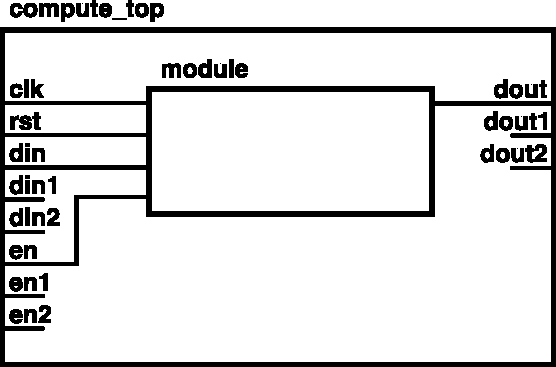
\includegraphics[width=3.5in]{compute_top.pdf}
\caption{compute\_top}
\label{fig:compute_top}
\end{center}
\end{figure}

In the TMR version we want the BL-TMR tool to triplicate the internals of the
design and wire up the second and third domains to the corresponding ports (i.e.
\texttt{din1} and \texttt{din2} correspond to the second and third domains for
\texttt{din}) as in Figure~\ref{fig:compute_top_tmr}.

\begin{figure}[htb]
\begin{center}
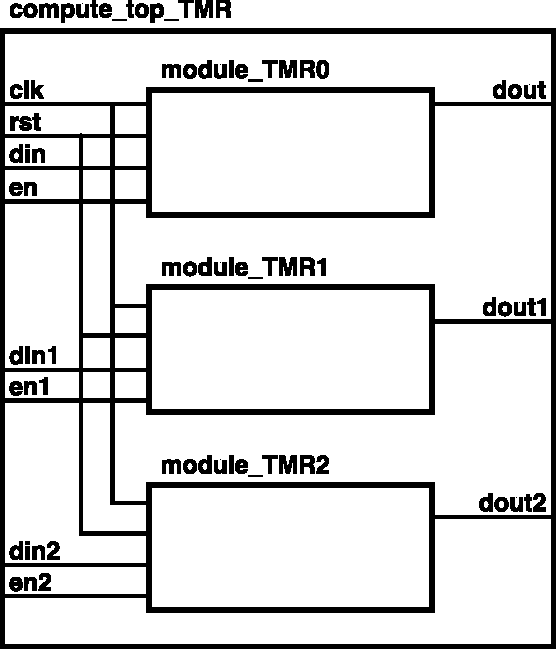
\includegraphics[width=3.5in]{compute_top_tmr.pdf}
\caption{compute\_top\_TMR}
\label{fig:compute_top_tmr}
\end{center}
\end{figure}

We can accomplish this by telling the tools about the port groupings (i.e.
\texttt{din}, \texttt{din1}, and \texttt{din2} form a port group). Each port
group has a replication type (one of \texttt{triplication} or
\texttt{duplication}) and a name. The name of a port group doesn't matter as
long as each port in the group has the same name. Each port in a port group has
an index. Each \texttt{triplication} port group must have three ports with
indices $0$, $1$, and $2$. Each \texttt{duplication} port group must have two
ports with indices $0$ and $1$. We tell the BL-TMR tool about our port groupings
through EDIF properties on the ports which can be generated using VHDL
attributes. The EDIF property should be named \texttt{port\_group} and should
be of type \texttt{string}. The format for the string is ``\texttt{<replication
type>:<port group name>:<port index>}''. For the \texttt{compute\_top} design
above, we would put the appropriate EDIF properties on the ports using the
following VHDL code:
\begin{verbatim}
entity compute_top is
  port (
    clk : in std_logic;
    rst : in std_logic;
    din : in std_logic_vector(7 downto 0);
    din1 : in std_logic_vector(7 downto 0);
    din2 : in std_logic_vector(7 downto 0);
    en : std_logic;
    en1 : std_logic;
    en2 : std_logic;
    dout : std_logic_vector(7 downto 0);
    dout1 : std_logic_vector(7 downto 0);
    dout2 : std_logic_vector(7 downto 0)
    );
	
    attribute port_group : string;

    attribute port_group of din : signal is "triplication:din:0";
    attribute port_group of din1 : signal is "triplication:din:1";
    attribute port_group of din2 : signal is "triplication:din:2";

    attribute port_group of en : signal is "triplication:en:0";
    attribute port_group of en1 : signal is "triplication:en:1";
    attribute port_group of en2 : signal is "triplication:en:2";

    attribute port_group of dout : signal is "triplication:dout:0";
    attribute port_group of dout1 : signal is "triplication:dout:1";
    attribute port_group of dout2 : signal is "triplication:dout:2";

end entity compute_top;
\end{verbatim}

Notice that the \texttt{clk} and \texttt{rst} signals do not have port group
attributes because we have chosen not to pre-triplicate these particular
signals. (We could still tell the BL-TMR tool to triplicate these ports, if
desired, by using the \texttt{--tmr\_p <port\_name>}). When the port group attributes
above are used in the VHDL code, the BL-TMR tool automatically wires the ports
to the appropriate domains after triplicating the design internals. Port groups can
also be used for pre-duplicated ports. A single design can use both
\texttt{triplication} and \texttt{duplication} port groups if desired.

\subsection{Pre-mitigated Components}
Pre-mitigated components are useful in situations where standard TMR with
bitstream scrubbing is not a sufficient mitigation strategy and alternative
mitigation strategies need to be implemented manually in certain portions of a
design before TMR is applied to the rest of the design. One such situation is
that of using a block RAM with a soft-core processor. Block RAMs are susceptible
to SEUs but bitstream scrubbing cannot correct errors in block BRAMs used as
RAM (not ROM) because there is no ``golden copy'' of the BRAM contents. A BRAM
scrubber can provide error correction in such a situation.

A TMR BRAM scrubber generally consists of three instances of a BRAM with
additional logic to repeatedly read the contents of the three BRAMs and correct
any bits where there is a discrepancy between the three copies. A BRAM scrubber
instantiates dual-ported BRAMs and uses one of the ports for scrubbing and
exposes the other port for normal access by the rest of the circuit.

Using a BRAM scrubber as a pre-mitigated component can simplify the process of
implementing TMR in the rest of the circuit. Consider a design that uses a
$4096$-bit single-port synchronous Block RAM with a port width of $4$
(RAMB$4$\_S$4$) as shown in Figure~\ref{fig:ramb4_s4}.

\begin{figure}[htb]
\begin{center}
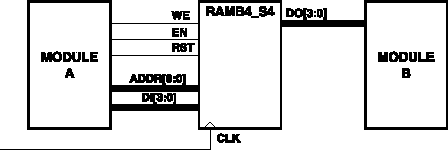
\includegraphics[scale=1]{ramb4_s4.pdf}
\caption{Design with Block RAM}
\label{fig:ramb4_s4}
\end{center}
\end{figure}

It is possible to develop a BRAM scrubber as a drop in replacement for the
single-port BRAM. Such a replacement would use three dual-ported BRAMs and
would expose all three TMR domains of one of the access ports to the rest of
the design as shown in Figure~\ref{fig:ramb4_s4_tmr}. For this example, we will
assume that we have developed such a scrubber.

\begin{figure}[htb]
\begin{center}
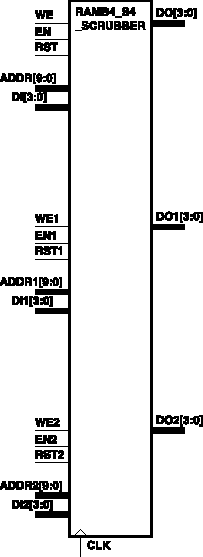
\includegraphics[scale=1]{ramb4_s4_tmr.pdf}
\caption{Block RAM Scrubber}
\label{fig:ramb4_s4_tmr}
\end{center}
\end{figure}

In this example, all signals have been triplicated except for the clock signal.
After replacing the original BRAM with the scrubber replacement we would have
the design shown in Figure~\ref{fig:ramb4_s4_tmr_design}. Notice that only the
first domain is wired for each signal since the rest of the design is still
untriplicated.

\begin{figure}[htb]
\begin{center}
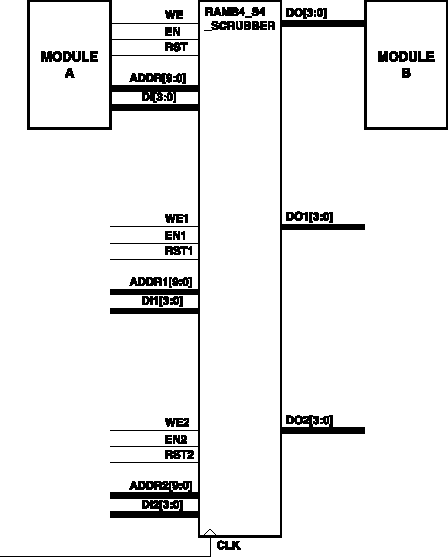
\includegraphics[scale=1]{ramb4_s4_tmr_design.pdf}
\caption{Design with Block RAM Scrubber}
\label{fig:ramb4_s4_tmr_design}
\end{center}
\end{figure}

By declaring port groups for the ports on the scrubber, we can tell the BL-TMR
tool how to wire up the unwired ports when the rest of the design gets
triplicated. As with pre-mitigated top-level ports, we do so by using VHDL
attributes. The entity declaration for our BRAM scrabber should be as follows:
\begin{verbatim}
entity RAMB4_S4_SCRUBBER
  port (
    WE : in std_logic;
    WE1 : in std_logic;
    WE2 : in std_logic;
    EN : in std_logic;
    EN1 : in std_logic;
    EN2 : in std_logic;
    RST : in std_logic;
    RST1 : in std_logic;
    RST2 : in std_logic;
    CLK : in std_logic;
    ADDR : in std_logic_vector(9 downto 0);
    ADDR1 : in std_logic_vector(9 downto 0);
    ADDR2 : in std_logic_vector(9 downto 0);
    DI : in std_logic_vector(3 downto 0);
    DI1 : in std_logic_vector(3 downto 0);
    DI2 : in std_logic_vector(3 downto 0);
    DO : out std_logic_vector(3 downto 0);
    DO1 : out std_logic_vector(3 downto 0);
    DO2 : out std_logic_vector(3 downto 0)
    );

  attribute port_group : string;

  attribute port_group of WE : signal is "triplication:WE:0";
  attribute port_group of WE1 : signal is "triplication:WE:1";
  attribute port_group of WE2 : signal is "triplication:WE:2";
  
  attribute port_group of EN : signal is "triplication:EN:0";
  attribute port_group of EN1 : signal is "triplication:EN:1";
  attribute port_group of EN2 : signal is "triplication:EN:2";

  attribute port_group of RST : signal is "triplication:RST:0";
  attribute port_group of RST1 : signal is "triplication:RST:1";
  attribute port_group of RST2 : signal is "triplication:RST:2";

  attribute port_group of ADDR : signal is "triplication:ADDR:0";
  attribute port_group of ADDR1 : signal is "triplication:ADDR:1";
  attribute port_group of ADDR2 : signal is "triplication:ADDR:2";

  attribute port_group of DI : signal is "triplication:DI:0";
  attribute port_group of DI1 : signal is "triplication:DI:1";
  attribute port_group of DI2 : signal is "triplication:DI:2";

  attribute port_group of DO : signal is "triplication:DO:0";
  attribute port_group of DO1 : signal is "triplication:DO:1";
  attribute port_group of DO2 : signal is "triplication:DO:2";
  
end entity RAMB4_S4_SCRUBBER;
\end{verbatim}

It should be noted that some care must be taken with synthesis tools in order
to preserve pre-mitigated components as separate components. Many synthesis
tools flatten some design hierarchy. When this happens to a pre-mitigated
component, the port declarations and port group properties are lost. The most
reliable way to prevent this is to leave pre-mitigated components as black
boxes in the main design and synthesize the pre-mitigated components separately
(making sure to disable IO buffer insertion). This results in a main EDIF
file for the top design component and a separate EDIF file for each
pre-mitigated component. The BL-TMR tool can merge the black boxes into the main
design while preserving port group properties if all of the EDIF files are
placed in the same directory or their paths are indicated using the appropriate
commandline options.

When the BL-TMR tool is used to apply TMR to the design in
Figure~\ref{fig:ramb4_s4_tmr_design} with the port group attributes shown above,
the resulting design gets all of the ports wired up to the appropriate domains
as shown in Figure~\ref{fig:ramb4_s4_tmr_result}.

\begin{figure}[htb]
\begin{center}
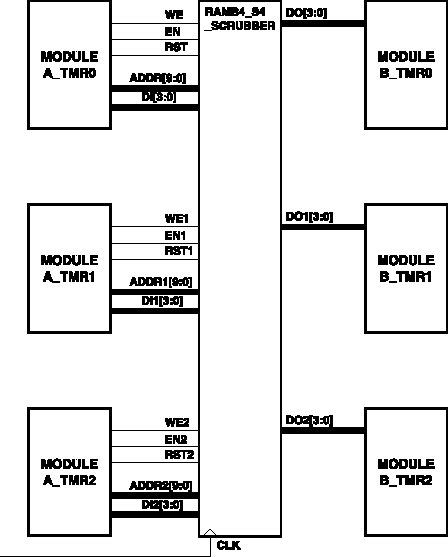
\includegraphics[scale=1]{ramb4_s4_tmr_result.pdf}
\caption{Triplicated Design with Block RAM Scrubber}
\label{fig:ramb4_s4_tmr_result}
\end{center}
\end{figure}

\subsection{Implementation Issues}
\subsubsection{VHDL Open Ports}
In order to create a design with unconnected ports such as that shown in
Figure~\ref{fig:ramb4_s4_tmr_design}, it is necessary to leave the unused
(i.e. second and third domain) ports \texttt{open} in the VHDL component
instantiation statement. Synthesis tools generally wire \texttt{open} ports
with no default value specified to \texttt{GND}. The BL-TMR tool removes any
connections on second and third domain ports of pre-mitigated components before
wiring them to the rest of the design in order to prevent input ports from
being driven by \texttt{GND} in addition to their correct drivers.

\subsubsection{Proprietary Pre-mitigated Cores}
Some core formats such as .ngc are proprietary and cannot be read by the BL-TMR
tool. When a pre-mitigated core is in a proprietary format, it can still be
used, however, because the BL-TMR tool simply works on the black box definition
of the core. All appropriate connections to the black box will be made and the
core can be merged in by proprietary tools after running the BL-TMR tool. The
only difficulty with this process is that any \texttt{port\_group} properties for
pre-mitigated proprietary cores must be inserted into the black box cell
definition in the main EDIF file manually because VHDL has no means of putting
attributes on component declaration ports.


\section{Common Usage of JEdifTMRAnyalysis}
This section describes a few sample scenarios and explains which combination of
command line options should be used for each.

%%%%%%%%%%%%%%%%%%%%%%%%%%%%%%%%%%%%%%%%%%%%%%
\subsection{Full TMR}
\label{subsec:fulltmr}
This example shows how to perform ``full'' TMR (triplication of all components) 
on a design. For larger designs, this may result in a TMR'd version of the 
design that does not fit in the desired chip. If this is the case, some form of 
``partial'' TMR should be used.

In this example, the design to be triplicated is specified in the file 
\texttt{myDesign.edf} and the triplicated design will be written to 
\texttt{myDesign\_tmr.edf}. Both input ports and output ports are triplicated. 
The part used in this case is the Virtex II XC2V1000-FG456.

\begin{verbatim}
> java edu.byu.ece.edif.jedif.JEdifTMRAnalysis myDesign.jedif \
  -o myDesign.ptmr -iob_output myDesign.iob\
  --tmr_inports --tmr_outports --full_tmr --technology Virtex2 --part xc2v1000fg456
\end{verbatim}


%%%%%%%%%%%%%%%%%%%%%%%%%%%%%%%%%%%%%%%%%%%%%%
\subsection{Full TMR---Clock not triplicated}
Some systems do not support triplicated clock lines. This example shows how to 
triplicate everything but the clock line.

This example is almost identical to the example in section 
\ref{subsec:fulltmr}. The \texttt{--no\_tmr\_p} option specifies that the 
top-level port named \texttt{Clk} (case-sensitive) should not be triplicated. 
The \texttt{--no\_tmr\_c} option indicates that all cells of the global clock 
buffer type \texttt{BUFG} should also not be triplicated. This prevents the 
clock line after the buffer from being triplicated and the entire circuit will 
use the same single clock.

\begin{verbatim}
> java edu.byu.ece.edif.jedif.JEdifTMRAnalysis myDesign.jedif \
  --tmr_inports --tmr_outports --full_tmr --no_tmr_p Clk --no_tmr_c BUFG \
  --technology  Virtex2 --part xc2v1000fg456
\end{verbatim}


%%%%%%%%%%%%%%%%%%%%%%%%%%%%%%%%%%%%%%%%%%%%%%
\subsection{Full TMR---No I/O triplication}
Many FPGA applications are port-limited. This example shows how to prevent all 
inputs and outputs from being triplicated. In this example, the user must leave 
out the \texttt{--tmr\_inports} and \texttt{--tmr\_outports} parameters so that 
top level ports are not included in triplication. This example also leaves out 
the \texttt{--technology} and \texttt{--part} options, using the default values 
for each (Virtex XCV1000-FG680).

\begin{verbatim}
> java edu.byu.ece.edif.jedif.JEdifTMRAnalysis myDesign.jedif --full_tmr
\end{verbatim}


%%%%%%%%%%%%%%%%%%%%%%%%%%%%%%%%%%%%%%%%%%%%%%
\subsection{Partial TMR---No I/O triplication}
This example shows a standard usage of the BL-TMR tool for partial TMR\@. In this 
case, the design is too large to fit in the targeted device when fully 
triplicated. The BL-TMR tool will triplicate as much logic as possible and 
estimate when the target chip will be fully utilized.

%This design also requires some external EDIF files that are referenced in 
%\texttt{myLargeDesign.edf} as ``black boxes.'' These external files, which are 
%located in the \texttt{externalSrcDir} directory, will be incorporated into the 
%triplicated design. Thus, the external files will not be needed with the 
%\texttt{myLargeDesign\_BL-TMR.edf} output file.

\begin{verbatim}
> java edu.byu.ece.edif.jedif.JEdifTMRAnalysis myLargeDesign.jedif 
\end{verbatim}


%%%%%%%%%%%%%%%%%%%%%%%%%%%%%%%%%%%%%%%%%%%%%%
\subsection{Partial TMR---SCC Decomposition, custom estimation factors}
In this case, the user wishes to include parts of strongly-connected components 
(SCCs) for triplication. This example also shows how to override the default
merge and optimization factors.

\begin{verbatim}
> java edu.byu.ece.edif.jedif.JEdifTMRAnalysis myLargeDesign.jedif 
  -d ./externalSrcDir --doSCCDecomposition --mergeFactor 0.4 --optimizationFactor 0.85
\end{verbatim}


%%%%%%%%%%%%%%%%%%%%%%%%%%%%%%%%%%%%%%%%%%%%%%
\subsection{Partial TMR---Fill 50\% of target device}
In some cases, the user may wish to use the triplicated design on the same chip 
as another design. In this example the user knows that a separate design will 
require half of the target chip. To fill as much of the left-over 50\% as 
possible, the user specifies a \texttt{--factor\_type} of \texttt{DUF} and a 
\texttt{factor\_value} of \texttt{0.5}. This will stop triplication of the 
input design when half of the target chip is utilized, according to the 
estimate made with the merge optimization factors.

\begin{verbatim}
> java edu.byu.ece.edif.jedif.JEdifTMRAnalysis myLargeDesign.jedif 
  --factor_type DUF --factor_value 0.5
\end{verbatim}


%%%%%%%%%%%%%%%%%%%%%%%%%%%%%%%%%%%%%%%%%%%%%%
\subsection{Partial TMR---Push utilization past 100\%}
Due to the way mapping tools are implemented, the user may be able to fit more 
logic onto the target chip than estimated by the utilization tracker. The 
Xilinx \texttt{map} program, for example, does not map unrelated logic into the 
same slice until slice utilization reaches 99\%. This means that much more 
logic can be added after this point, though the place and route step will 
become increasingly more difficult for the tools to perform.

With this in mind, to achieve the maximum capacity on the target chip, it may 
be necessary to specify a desired utilization factor greater than 1.0 (more 
than 100\% estimated utilization). The following example uses a device 
utilization factor of 1.5, which will stop triplication when an estimated 150\% 
of the target part is utilized.

\begin{verbatim}
> java edu.byu.ece.edif.jedif.JEdifTMRAnalysis myLargeDesign.jedif \
  --factor_type DUF --factor_value 1.5
\end{verbatim}


%%%%%%%%%%%%%%%%%%%%%%%%%%%%%%%%%%%%%%%%%%%%%%
\subsection{Partial TMR---Use 75\% of available space on target device}
The available space utilization factor can be used to specify the amount of
space on the target device left after the unmitigated circuit is mapped. To
fill the chip up to 75\% of the left-over space, the user specifies a 
\texttt{--factor\_type} of \texttt{ASUF} and a \texttt{factor\_value} of 
\texttt{0.75}. If the original design size is estimated at using 40\% of the
target chip, this will stop triplication when 70\% ($40 + (100-40)*0.75$) of
the target chip is utilized.

\begin{verbatim}
> java edu.byu.ece.edif.jedif.JEdifTMRAnalysis myLargeDesign.jedif 
   --factor_type DUF --factor_value 0.5
\end{verbatim}


%%%%%%%%%%%%%%%%%%%%%%%%%%%%%%%%%%%%%%%%%%%%%%
\subsection{Using Configuration Files}
\label{using config}
Configuration files can greatly simplify the use of any of the
 BL-TMR tools.  The following examples show how to create and use
 configuration files. (See section \ref{config options},
 ``Configuration File Options'' for more information.)

\subsubsection{Create a Configuration File}
The following will write the current command-line arguments to the file
\texttt{myConfig.conf}:

\begin{verbatim}
> java edu.byu.ece.edif.jedif.JEdifTMRAnalysis myDesign.edf -o myDesign_BL-TMR.edf -f \ 
subcell.edf,/usr/share/edifFiles/subcell2.edf, -d /usr/share/edif/common/ \ 
--tmr_inports --tmr_outports --tmr_c DLL,fdc,clk_buf --tmr_i clk,fifo_output \ 
--no_tmr_p clk_port,data_in --no_tmr_c bufg --no_tmr_i mux2,and24 \ 
--notmrFeedForward --inputAdditionType 1 --outputAdditionType 2 --mergeFactor \ 
0.85 --optimizationFactor 0.90 --technology Virtex2 --part XCV1000FG680 --log myLogFile.log \
--writeConfig:myConfig.conf
\end{verbatim}

The previous command creates the following output, stored in 
\texttt{myConfig.conf}:

\begin{verbatim}
#myConfig.conf, created by edu.byu.ece.edif.util.jsap.NMRCommandParser
#Sat Jul 22 19:51:14 MDT 2006
hlUsePort=hl_port
availableSpaceUtilizationFactor=0.85
tmr_c=DLL,fdc,clk_buf
summary=true
optimizationFactor=0.9
log=myLogFile.log
notmrFeedForward=true
output=myDesign_BL-TMR.edf
hlConst=0
input=myDesign.edf
outputAdditionType=2
mergeFactor=0.85
removeHL=true
dir=/usr/share/edif/common/
writeConfig=myConfig.conf
part=XCV1000FG680
no_tmr_p=clk_port,data_in
technology=Virtex2
domainReport=myDomainReport.txt
inputAdditionType=1
no_tmr_i=mux2,and24
file=subcell.edf,/usr/share/edifFiles/subcell2.edf
no_tmr_c=bufg
tmr_i=clk,fifo_output
tmr_outports=true
tmr_inports=true
\end{verbatim}

Configuration files are defined by the \texttt{java.util.Properties} class. 
However, the format is simple enough that configuration files can easily be 
created by hand or by other programs. As seen above, the format is simply 
\texttt{key=value}. A hash mark (pound sign) (\texttt{\#}) at the beginning of 
a line marks that line as a comment. BL-TMR options are given just as they would 
be on the command-line, with the exception that command-line options with no 
arguments (e.g. \texttt{--tmr\_inports}, \texttt{--summary}, 
\texttt{--doSCCDecomposition}, etc.) are specified as either \texttt{true} or 
\texttt{false}, as seen above.

\subsubsection{Use a Configuration File}

The following example shows how to load \texttt{myConfig.conf} as a configuration
file:

\begin{verbatim}
> java edu.byu.ece.edif.jedif.JEdifTMRAnalysis --useConfig myConfig.conf
\end{verbatim}

\subsubsection{Combining Configuration Files and Command-line Arguments}
Configuration files provide default values of BL-TMR options. Any options 
specified on the command-line will take precedence. (See section 
\ref{useConfig}, ``\texttt{--useConfig}'' for detailed precedence information.)
The following example uses the same options specified by myConfig.conf, but
changes the input and output files:

\begin{verbatim}
> java edu.byu.ece.edif.jedif.JEdifTMRAnalysis myOtherDesign.edf -o myOtherDesign_BL-TMR.edf \
 --useConfig myConfig.conf
\end{verbatim}

%%%%%%%%%%%%%%%%%%%%%%%%%%%%%%%%%%%%%%%%%%%%%%%%%%%%%%%%%%%%

\newpage
\section{Sample Makefile for TMR}
\verbatimtabinput{makefile_tmr}
\newpage
\section{Sample Makefile for DWC}
\verbatimtabinput{makefile_dwc}
\newpage
\section{Sample Makefile for mixed TMR/DWC}
\verbatimtabinput{makefile_tmr_dwc}


%%%%%%%%%%%%%%%%%%%%%%%%%%%%%%%%%%%%%%%%%%%%%%

%%%%%%%%%%%%%%%%%%%%%%%%%%%%%%%%%%%%%%%%%%%%%%%%%%%%%%%%%%%%
\newpage
\section{Special Notes}

%%%%%%%%%%%%%%%%%%%%%%%%%%%%%%%%%%%%%%%%%%%%%%
\subsection{Naming Conventions}
\label{naming conventions}
The BL-TMR tool alters the names of replicated signals, cell instances, and 
ports. Be aware of this when using placement (or other) constraints. An output
port named \texttt{myOutport} in the original EDIF file, when triplicated,
would become \texttt{myOutport\_TMR\_0}, \texttt{myOutport\_TMR\_1}, and
\texttt{myOutport\_TMR\_2}. When duplicated, the output port would become
\texttt{myOutport\_DWC\_0} and \texttt{myOutport\_DWC\_1}. Similarly, a
flip-flop whose instance name is \texttt{myFF} in the original file, when
triplicated, would become \texttt{myFF\_TMR\_0}, \texttt{myFF\_TMR\_1}, and
\texttt{myFF\_TMR\_2}. When duplicated, the instance would become
\texttt{myFF\_DWC\_0} and \texttt{myFF\_DWC\_1}. Net names follow the same
convention.

%%%%%%%%%%%%%%%%%%%%%%%%%%%%%%%%%%%%%%%%%%%%%%
\subsection{Allocating More Memory for the JVM}
Larger designs may require more heap memory than the Java Virtual Machine (JVM) 
is allocated by default. Use the \texttt{-Xmx}
\footnote{See 
\url{http://java.sun.com/j2se/1.5.0/docs/tooldocs/windows/java.html\#Xms} 
for more information about this and other command-line options to the JVM.} 
option with the Java executable to change the maximum amount of memory for 
the virtual machine. The following example allocates up to 256 MB of 
heap space for the JVM:

\begin{verbatim}
> java -Xmx256M byucc.edif.tools.tmr.FlattenTMR ...
\end{verbatim}

%%%%%%%%%%%%%%%%%%%%%%%%%%%%%%%%%%%%%%%%%%%%%%%%%%%%%%%%%%%%
\section{Change Log}

\subsection*{Version 0.4.0 - 30 May 2008}
\begin{itemize}
\item Moved ChangeLog out of this file. Please see the file
edu.byu.ece.edif.doc.CHANGE\_LOG.txt for more information.
\end{itemize}

\subsection*{Version 0.3.4 - No official release date}
\begin{itemize}
\item Fixed --hl\_use\_port option on JEdifSterilize (was --hl\_port\_name)
\item Rearranged and added sections of this document
\item Made –remove\_fmaps option to default to false
\item Fixed bug in EdifCell.deleteSubCell(EdifCellInstance, boolean) in 
which referenced EdifNets were not removed when requested
\end{itemize}

\subsection*{Version 0.3.3 - 15 Jan 2008}
\begin{itemize}
\item Fixed bug involving source-to-source edges in
EdifCellInstanceConnectivity. This had caused IOB registers to not be recognized
correctly.
\item Fixed bug in which Virtex II parts were incorrectly rejected by the tool
\item Added SRL Replacement to JEdifBuild
\item BLDWC now has the option to separate detection between persistent and
non-persistent
\end{itemize}

\subsection*{Version 0.3.2 - 24 Aug 2007}
\begin{itemize}
\item Various minor bug fixes
\end{itemize}

\subsection*{Version 0.3.1 - 14 Aug 2007}
\begin{itemize}
\item Fixed issues with BRAM and DSP blocks
\item BLTMR can now extract the part number if included in the input EDIF file.
\item Fixed bug in which a triplicated clock line could be voted on.
\item Fixed bug in which DLLs were not recognized.
\end{itemize}

\subsection*{Version 0.3.0 - 16 Jul 2007}
\begin{itemize}
\item Split TMR into several tools
\item TMR tool flow now uses jedif files
\item Added clock domain analysis tools
\item Added more frequent voting tool
\end{itemize}

\subsection*{Version 0.2.4 - 16 Feb 2007}
\begin{itemize}
\item Fixed bugs in EdifHalfLatchRemover: 
\begin{itemize}
\item Added support for BlackBox modules
\item Removed addition of ``\_hl'' suffix to replaced primitives
\end{itemize}
\item Added option to allow user to specify suffixes for triplicated design
elements
\item Design name in output file now matches top-level Cell
\item Fixed bug in SCCUtilities
\item created new HalfLatchFlattenedEdifCell class, tool now flattens before HL
removal
\item HL removal now recognizes IOB registers
\item Added option to ignore feedback through IOBs
\item Port components are automatically triplicated/not triplicated with the port
\end{itemize}

\subsection*{Version 0.2.3 - 12 Oct 2006}
\begin{itemize}
\item Fixed bug when writing config files
\item Fixed bug in SCC code that could cause a ConcurrentModificationException
\item Fixed bug in which BL-TMR could produce an invalid design due to too many
  connections to a MUXF6 input
\end{itemize}

\subsection*{Version 0.2.2 - 25 Sep 2006}
\begin{itemize}
  \item User may now specify hierarchical instance names for forced inclusion
  in/exclusion from TMR
  \item Added Half-Latch Removal as a command-line option
  \item Now using NMREdifCell instead of TMREdifCell, which slightly changed the
  naming policy for triplicated elements (See section \ref{naming conventions}
  ``Naming Conventions'')
  \item Added fmap removal (fixes the use of inputAdditionType=1)
  \item Added Multiple EDIF Creation
  \begin{itemize}
    \item Removed the DUF, UEF, and ASUF command-line parameters
    \item Added factor\_type and factor\_value command-line parameters
  \end{itemize}
\end{itemize}

\subsection*{Version 0.2.1 - 28 Jul 2006}
\begin{itemize}
\item Now disallows voting between MUXF5, MUXF6, MUXF7, MUXF8
\item Added unused cell trimming
\end{itemize}

\subsection*{Version 0.2.0 - 25 Jul 2006}
\begin{itemize}
\item New command-line parser\footnote{The BL-TMR tool uses \emph{JSAP: the 
Java-based Simple Argument Parser} by Martian Software, Inc.\ for parsing 
command-line arguments.  JSAP and its source code can be found at 
\url{http://www.martiansoftware.com/jsap/index.html}.} (not backwards 
compatible)
\item Added half-latch removal option
\item Added configuration files support
\item Some command-line parameters have been renamed
\item Added recursive black box merging
\item Fixed bug which caused some nets to lose their original name
\end{itemize}

\subsection*{Version 0.1.9 - 3 Jul 2006}
\begin{itemize}
\item Fixed bug in which output EDIF file could be invalid and crash in the map 
stage (voters were inserted in the carry chain).
\end{itemize}

\subsection*{Version 0.1.8 - 13 Jun 2006}
\begin{itemize}
\item Added triplication status to reports
\item Added available space utilization factor
\item Added force triplicate options
\item Fixed bug in SCCUtilities that could cause a class cast exception
\end{itemize}

\subsection*{Version 0.1.7 - 23 May 2006}
\begin{itemize}
\item Added DLLs to resources tracked for Virtex parts
\item Added options for ordering of SCC additions (-SCCSortType)
\end{itemize}

\subsection*{Version 0.1.6 - 18 May 2006}
\begin{itemize}
\item Added options to select type of partial Input to Feedback and Feedback 
Output addition to TMR (-input and -outputAdditionType)
\item Added option to ignore INOUT port restriction
\item Moved to Java 5
\end{itemize}

\subsection*{Version 0.1.5 - 12 May 2006}
\begin{itemize}
\item Version 0.1.4 contained a left-over debug printout. This was removed.
\end{itemize}

\subsection*{Version 0.1.4 - 11 May 2006}
\begin{itemize}
\item Added option for naming tmr domain report
\item Added utilization\_expansion\_factor option
\end{itemize}

\subsection*{Version 0.1.3 - 3 May 2006}
\begin{itemize}
\item Added options to selectively exclude Feedback, Input to Feedback, 
Feedback Output, and Feed-forward sections from TMR.
\item Complete partial TMR now matches ``Full'' TMR\@. (Before this, the 
``Feed-forward'' section was not included.)
\end{itemize}

\subsection*{Version 0.1.2 - 17 Apr 2006}
\begin{itemize}
\item Added automatic IOB handling. The user no longer needs to specifically 
include or exclude IBUFs, OBUFs, etc.
\item Added automatic log file creation. The user may also customize the 
filename of the logfile.
\item Fixed issue in which ``rename'' directives in the original EDIF were not 
preserved. The output EDIF now contains the original ``rename''s.
\end{itemize}

\subsection*{Version 0.1.1 - 9 Mar 2006}
\begin{itemize}
\item Added version number to the output of the tool for version tracking
purposes.
\end{itemize}

\subsection*{Initial Release---Version 0.1.0 - 8 Mar 2006}
\begin{itemize}
\item Initial release outside of BYU\@. No version number is contained in
the released JAR file.
\end{itemize}

\end{document}

%
% Words to be ignored by the spell-checker:
%

% LocalWords:  BYU LANL BL-TMR EDIF FPGA TMR OBUF IBUF BUFG IBUFG LUTs
% LocalWords:  SCC SCCs FFs UCF Xilinx java JHDL netlister IOB IBUFs
% LocalWords:  OBUFs logfile INOUT TMR'd tmr txt 

